% =========================
% CHAPITRE 2 : ANALYSE ET ARCHITECTURE DU SYSTÈME
% Fichier a inclure depuis le rapport principal via % =========================
% CHAPITRE 2 : ANALYSE ET ARCHITECTURE DU SYSTÈME
% Fichier a inclure depuis le rapport principal via % =========================
% CHAPITRE 2 : ANALYSE ET ARCHITECTURE DU SYSTÈME
% Fichier a inclure depuis le rapport principal via % =========================
% CHAPITRE 2 : ANALYSE ET ARCHITECTURE DU SYSTÈME
% Fichier a inclure depuis le rapport principal via \input{chapters/chapitre2_analyse_systeme_architecture}
% =========================

\chapter{Analyse du système et architecture technique}
\label{chap:analyse_architecture}

\section{Introduction}
Ce chapitre formalise la vision système de la plateforme de dépistage automatisé de la rétinopathie diabétique.
Il présente d'abord l'analyse du système (acteurs, exigences), puis la modélisation UML globale,
et enfin l'architecture complete de la solution (logicielle, materielle et operationnelle).

Le contenu est appliqué au projet réalisé, en conservant les rôles métier réels :
\textbf{Administrateur de centre}, \textbf{Admin}, \textbf{Médecin}, \textbf{Super administrateur}, ainsi que l'acteur technique secondaire \textbf{Service IA}.

\section{Analyse du système}

\subsection{Acteurs}
Les acteurs identifiés sont classés en deux catégories : acteurs humains (métier) et acteurs système (techniques).

\subsubsection*{Acteurs humains (Human Actors)}
\begin{itemize}
    \item \textbf{Administrateur de centre} : gère les patients et les médecins du centre, crée les examens,
    envoie les images rétiniennes et consulte l'historique.
    \item \textbf{Admin} : assure l'administration applicative courante (parametrage, suivi operationnel,
    controle des utilisateurs selon les droits attribues).
    \item \textbf{Médecin} : consulte les examens classes par priorite, interprete la prediction IA et la heatmap,
    puis valide la conduite clinique.
    \item \textbf{Super administrateur} : administre les centres, gère la gouvernance globale (comptes, support, supervision,
    disponibilité du système).
\end{itemize}

\subsubsection*{Acteurs système (System Actors)}
\begin{itemize}
    \item \textbf{Service IA} (acteur secondaire principal) : reçoit l'image, exécute l'inférence,
    génère la heatmap Grad-CAM et retourne grade + confiance.
    \item \textbf{Service WebSocket} : diffuse les notifications temps reel (nouveaux examens, alertes severes,
    mises a jour d'etat).
    \item \textbf{Serveur SMTP/SMS} : assure les communications asynchrones (notifications, alertes critiques).
\end{itemize}

\textbf{Note de modelisation :} \textit{Patient} et \textit{Center} ne sont pas des acteurs,
mais des entités métier manipulées par les acteurs humains.

\subsection{Exigences fonctionnelles}
Les exigences fonctionnelles du système sont regroupées par domaine métier.

\subsubsection*{Gestion des comptes et sécurité}
\begin{itemize}
    \item authentification par rôle (Administrateur de centre, Admin, Médecin, Super administrateur) ;
    \item autorisation basée sur le rôle pour chaque route métier ;
    \item gestion de session et deconnexion sécurisée.
\end{itemize}

\subsubsection*{Gestion operationnelle du depistage}
\begin{itemize}
    \item création/modification/consultation/archivage de patients ;
    \item gestion des médecins rattachés à un centre ;
    \item création d'un examen avec téléversement d'image rétinienne ;
    \item association patient-médecin-centre lors de la création d'examen.
\end{itemize}

\subsubsection*{Analyse IA et explicabilité}
\begin{itemize}
    \item envoi de l'image vers le service IA ;
    \item prédiction automatique du grade de rétinopathie (0 à 4) ;
    \item calcul du score de confiance ;
    \item génération et stockage d'une heatmap Grad-CAM ;
    \item restitution du résultat dans l'interface Médecin.
\end{itemize}

\subsubsection*{Alertes et supervision}
\begin{itemize}
    \item création automatique d'alerte pour les cas sévères (grade $\geq 3$) ;
    \item notification temps réel du Médecin ;
    \item suivi de l'état des alertes (nouvelle, en cours, résolue) ;
    \item supervision transversale des centres et du support par le Super administrateur.
\end{itemize}

\subsection{Exigences non fonctionnelles}
Les exigences non fonctionnelles assurent la qualité globale du système en production.

\begin{itemize}
    \item \textbf{Performance} : temps de reponse court pour l'inference et l'affichage ;
    \item \textbf{Disponibilité} : accès continu des interfaces centre, médecin et supervision ;
    \item \textbf{Sécurité} : protection des données médicales, contrôle d'accès et isolation par centre ;
    \item \textbf{Fiabilité} : traçabilité des examens, alertes et actions utilisateurs ;
    \item \textbf{Scalabilite} : possibilite d'augmenter le nombre de centres et le volume d'images ;
    \item \textbf{Maintenabilite} : architecture modulaire (frontend, backend, IA, realtime) ;
    \item \textbf{Explicabilité} : visualisation interprétable (Grad-CAM) pour appuyer la décision clinique.
\end{itemize}

\section{Modélisation du système}

\subsection{Diagramme de cas d'utilisation général}
Le diagramme suivant represente la vue fonctionnelle globale avec
quatre acteurs primaires (Administrateur de centre, Admin, Médecin, Super administrateur) et un acteur secondaire (Service IA).

\begin{figure}[H]
\centering
\begin{tikzpicture}[scale=0.86, every node/.style={font=\small}]
    % Limite système
    \draw[thick] (1.8,0.6) rectangle (13.0,8.4);
    \node[anchor=west] at (2.0,8.1) {Système de dépistage RD};

    % Acteurs gauche
    % Administrateur de centre
    \draw (0.3,6.7) circle (0.25);
    \draw (0.3,6.45) -- (0.3,5.7);
    \draw (-0.2,6.05) -- (0.8,6.05);
    \draw (0.3,5.7) -- (-0.05,5.1);
    \draw (0.3,5.7) -- (0.65,5.1);
    \node at (0.3,4.8) {Administrateur de centre};

    % Admin
    \draw (-1.0,4.8) circle (0.25);
    \draw (-1.0,4.55) -- (-1.0,3.8);
    \draw (-1.5,4.15) -- (-0.5,4.15);
    \draw (-1.0,3.8) -- (-1.35,3.2);
    \draw (-1.0,3.8) -- (-0.65,3.2);
    \node at (-1.0,2.9) {Admin};

    % Médecin
    \draw (0.3,4.2) circle (0.25);
    \draw (0.3,3.95) -- (0.3,3.2);
    \draw (-0.2,3.55) -- (0.8,3.55);
    \draw (0.3,3.2) -- (-0.05,2.6);
    \draw (0.3,3.2) -- (0.65,2.6);
    \node at (0.3,2.3) {Médecin};

    % Super administrateur
    \draw (0.3,1.8) circle (0.25);
    \draw (0.3,1.55) -- (0.3,0.8);
    \draw (-0.2,1.15) -- (0.8,1.15);
    \draw (0.3,0.8) -- (-0.05,0.25);
    \draw (0.3,0.8) -- (0.65,0.25);
    \node at (0.3,-0.05) {Super administrateur};

    % Acteur secondaire droite : Service IA
    \draw (14.4,4.4) circle (0.25);
    \draw (14.4,4.15) -- (14.4,3.4);
    \draw (13.9,3.8) -- (14.9,3.8);
    \draw (14.4,3.4) -- (14.05,2.8);
    \draw (14.4,3.4) -- (14.75,2.8);
    \node at (14.4,2.45) {Service IA};

    % Use cases
    \node[draw, ellipse, minimum width=4.7cm, minimum height=0.85cm] (u1) at (5.5,7.3) {Se connecter};
    \node[draw, ellipse, minimum width=4.7cm, minimum height=0.85cm] (u2) at (5.5,6.2) {Gérer patients};
    \node[draw, ellipse, minimum width=4.7cm, minimum height=0.85cm] (u3) at (5.5,5.1) {Gérer médecins};
    \node[draw, ellipse, minimum width=4.7cm, minimum height=0.85cm] (u4) at (5.5,4.0) {Créer examen};
    \node[draw, ellipse, minimum width=4.7cm, minimum height=0.85cm] (u5) at (5.5,2.9) {Consulter historique};
    \node[draw, ellipse, minimum width=4.7cm, minimum height=0.85cm] (u6) at (9.4,5.8) {Consulter examens et alertes};
    \node[draw, ellipse, minimum width=4.7cm, minimum height=0.85cm] (u7) at (9.4,4.5) {Interpreter prediction + heatmap};
    \node[draw, ellipse, minimum width=4.7cm, minimum height=0.85cm] (u8) at (9.4,3.2) {Superviser centres et support};
    \node[draw, ellipse, minimum width=4.7cm, minimum height=0.85cm] (u9) at (9.4,1.9) {Administrer comptes globaux};
    \node[draw, ellipse, minimum width=4.7cm, minimum height=0.85cm] (u10) at (7.5,0.95) {Se déconnecter};
    \node[draw, ellipse, minimum width=4.7cm, minimum height=0.85cm] (u11) at (11.0,6.95) {Analyser image rétinienne};

    % Liens Administrateur de centre
    \draw (0.8,6.05) -- (u1.west);
    \draw (0.8,6.05) -- (u2.west);
    \draw (0.8,6.05) -- (u3.west);
    \draw (0.8,6.05) -- (u4.west);
    \draw (0.8,6.05) -- (u5.west);
    \draw (0.8,6.05) -- (u10.west);

    % Liens Médecin
    \draw (0.8,3.55) -- (u1.west);
    \draw (0.8,3.55) -- (u6.west);
    \draw (0.8,3.55) -- (u7.west);
    \draw (0.8,3.55) -- (u10.west);

    % Liens Admin
    \draw (-0.5,4.15) -- (u1.west);
    \draw (-0.5,4.15) -- (u2.west);
    \draw (-0.5,4.15) -- (u3.west);
    \draw (-0.5,4.15) -- (u5.west);
    \draw (-0.5,4.15) -- (u10.west);

    % Liens Super administrateur
    \draw (0.8,1.15) -- (u1.west);
    \draw (0.8,1.15) -- (u8.west);
    \draw (0.8,1.15) -- (u9.west);
    \draw (0.8,1.15) -- (u10.west);

    % Include vers IA
    \draw[->, dashed] (u4.east) -- (u11.west);
    \node at (8.6,6.6) {<<include>>};
    \draw[->, dashed] (u7.north) -- (u11.south);
    \node at (10.3,5.9) {<<include>>};

    % Lien acteur IA
    \draw (13.9,3.8) -- (u11.east);
\end{tikzpicture}
\caption{Diagramme de cas d'utilisation général du système.}
\label{fig:usecase_general_ch2}
\end{figure}

\subsection{Diagramme de classes general}
Le diagramme de classes ci-dessous montre les principales entités métier,
les specialisations de l'utilisateur et les relations entre objets applicatifs

\begin{figure}[H]
\centering
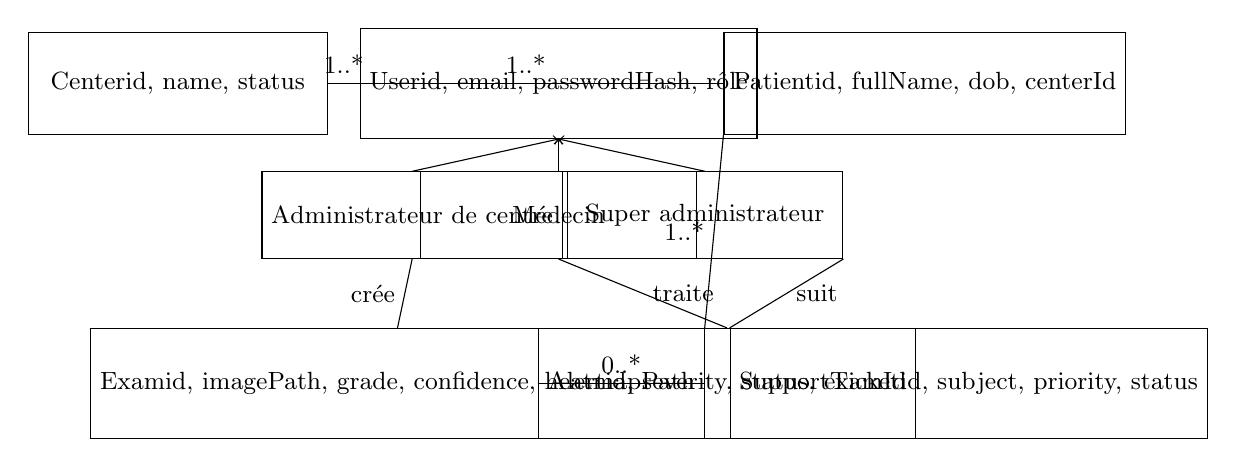
\begin{tikzpicture}[scale=0.93, every node/.style={font=\small}]
    % Classes principales
    \node[draw, rectangle, minimum width=3.8cm, minimum height=1.3cm] (center) at (2.0,7.0) {Center\\id, name, status};
    \node[draw, rectangle, minimum width=3.8cm, minimum height=1.4cm] (user) at (7.2,7.0) {User\\id, email, passwordHash, rôle};
    \node[draw, rectangle, minimum width=3.8cm, minimum height=1.3cm] (patient) at (12.2,7.0) {Patient\\id, fullName, dob, centerId};

    \node[draw, rectangle, minimum width=3.5cm, minimum height=1.1cm] (ca) at (5.2,5.2) {Administrateur de centre};
    \node[draw, rectangle, minimum width=3.5cm, minimum height=1.1cm] (doc) at (7.2,5.2) {Médecin};
    \node[draw, rectangle, minimum width=3.5cm, minimum height=1.1cm] (sa) at (9.2,5.2) {Super administrateur};

    \node[draw, rectangle, minimum width=4.0cm, minimum height=1.4cm] (exam) at (5.0,2.9) {Exam\\id, imagePath, grade, confidence, heatmapPath};
    \node[draw, rectangle, minimum width=4.0cm, minimum height=1.4cm] (alert) at (9.5,2.9) {Alert\\id, severity, status, examId};
    \node[draw, rectangle, minimum width=4.3cm, minimum height=1.4cm] (ticket) at (12.8,2.9) {SupportTicket\\id, subject, priority, status};

    % Relations
    \draw (center.east) -- node[above] {1..*} (user.west);
    \draw (center.east) -- node[above] {1..*} (patient.west);

    % Generalisation
    \draw[->] (ca.north) -- (user.south);
    \draw[->] (doc.north) -- (user.south);
    \draw[->] (sa.north) -- (user.south);

    \draw (patient.south west) -- node[left] {1..*} (exam.north east);
    \draw (ca.south) -- node[left] {crée} (exam.north);
    \draw (doc.south) -- node[right] {traite} (alert.north);
    \draw (exam.east) -- node[above] {0..*} (alert.west);
    \draw (sa.south east) -- node[right] {suit} (ticket.north west);
\end{tikzpicture}
\caption{Diagramme de classes general de la plateforme.}
\label{fig:class_general_ch2}
\end{figure}

\section{Architecture complète du système}

\subsection{Architecture du système (schéma global)}
Le schema global presente les couches logiques principales et les flux inter-services.

\begin{figure}[H]
\centering
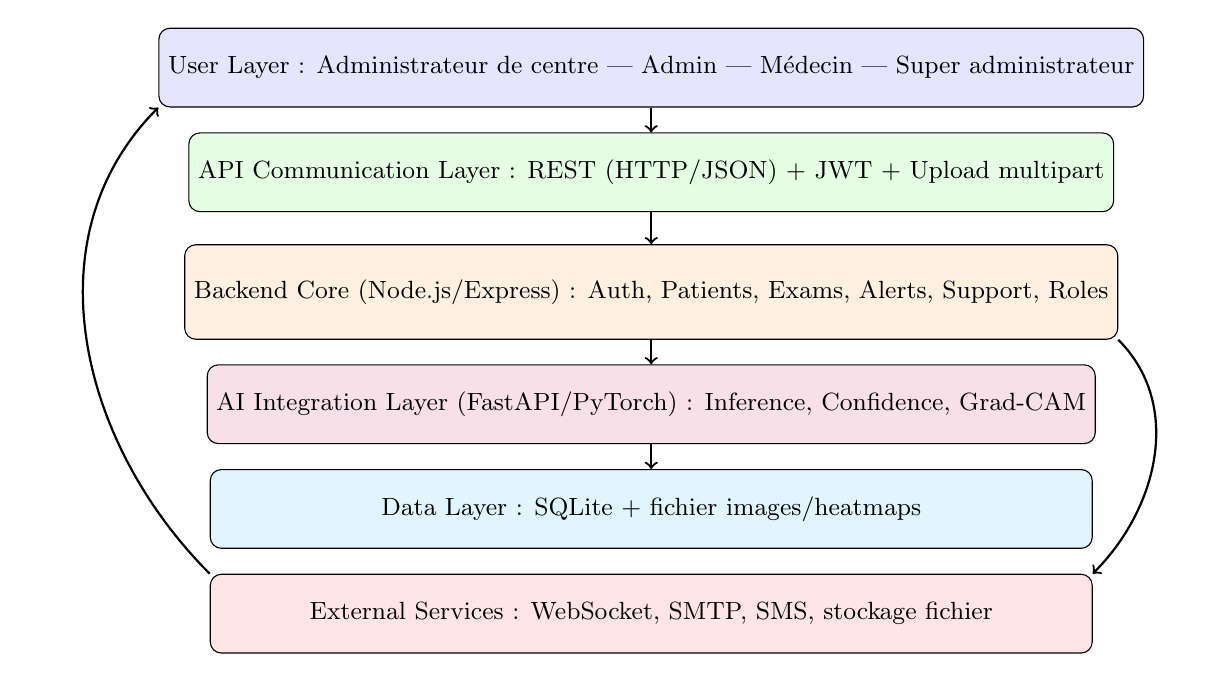
\begin{tikzpicture}[scale=0.95, every node/.style={font=\small}]
    \node[draw, rounded corners, fill=blue!10, minimum width=11.2cm, minimum height=1.0cm] (u) at (7.0,8.0) {User Layer : Administrateur de centre | Admin | Médecin | Super administrateur};
    \node[draw, rounded corners, fill=green!10, minimum width=11.2cm, minimum height=1.0cm] (api) at (7.0,6.6) {API Communication Layer : REST (HTTP/JSON) + JWT + Upload multipart};
    \node[draw, rounded corners, fill=orange!12, minimum width=11.2cm, minimum height=1.2cm] (core) at (7.0,5.0) {Backend Core (Node.js/Express) : Auth, Patients, Exams, Alerts, Support, Roles};
    \node[draw, rounded corners, fill=purple!12, minimum width=11.2cm, minimum height=1.0cm] (ai) at (7.0,3.5) {AI Integration Layer (FastAPI/PyTorch) : Inference, Confidence, Grad-CAM};
    \node[draw, rounded corners, fill=cyan!12, minimum width=11.2cm, minimum height=1.0cm] (data) at (7.0,2.1) {Data Layer : SQLite + fichier images/heatmaps};
    \node[draw, rounded corners, fill=red!10, minimum width=11.2cm, minimum height=1.0cm] (ext) at (7.0,0.7) {External Services : WebSocket, SMTP, SMS, stockage fichier};

    \draw[->, thick] (u.south) -- (api.north);
    \draw[->, thick] (api.south) -- (core.north);
    \draw[->, thick] (core.south) -- (ai.north);
    \draw[->, thick] (ai.south) -- (data.north);
    \draw[->, thick] (core.south east) to[out=-45,in=45] (ext.north east);
    \draw[->, thick] (ext.north west) to[out=135,in=-135] (u.south west);
\end{tikzpicture}
\caption{Schéma global de l'architecture du système.}
\label{fig:archi_globale_ch2}
\end{figure}

\subsection{Architecture globale de la plateforme}
L'architecture globale du système suit un enchaînement simple et lisible : les utilisateurs accèdent à l'interface web, les requêtes passent par l'API du backend, le service IA traite les images rétiniennes, puis les données et résultats sont stockés et diffusés aux différents rôles.

\begin{figure}[H]
\centering
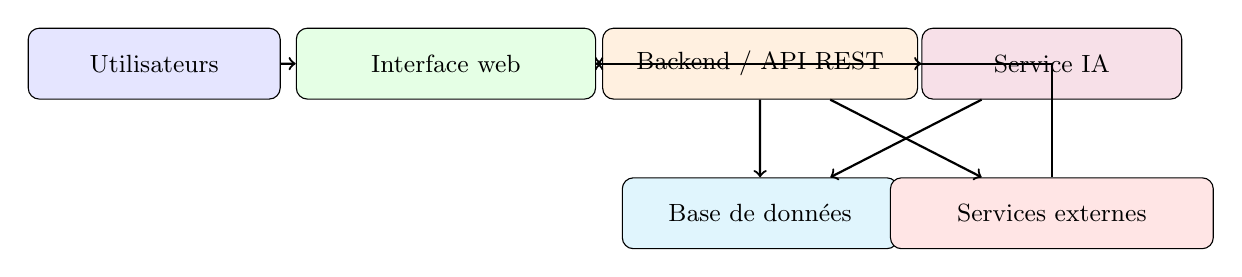
\begin{tikzpicture}[scale=0.95, every node/.style={font=\small}]
    \node[draw, rounded corners, fill=blue!10, minimum width=3.2cm, minimum height=0.9cm] (user) at (1.8,4.0) {Utilisateurs};
    \node[draw, rounded corners, fill=green!10, minimum width=3.8cm, minimum height=0.9cm] (front) at (5.7,4.0) {Interface web};
    \node[draw, rounded corners, fill=orange!12, minimum width=4.0cm, minimum height=0.9cm] (back) at (9.9,4.0) {Backend / API REST};
    \node[draw, rounded corners, fill=purple!12, minimum width=3.3cm, minimum height=0.9cm] (ai) at (13.8,4.0) {Service IA};

    \node[draw, rounded corners, fill=cyan!12, minimum width=3.5cm, minimum height=0.9cm] (data) at (9.9,2.0) {Base de données};
    \node[draw, rounded corners, fill=red!10, minimum width=4.1cm, minimum height=0.9cm] (ext) at (13.8,2.0) {Services externes};

    \draw[->, thick] (user) -- (front);
    \draw[->, thick] (front) -- (back);
    \draw[->, thick] (back) -- (ai);
    \draw[->, thick] (back) -- (data);
    \draw[->, thick] (back) -- (ext);
    \draw[->, thick] (ai) -- (data);
    \draw[->, thick] (ext) |- (front);
\end{tikzpicture}
\caption{Schéma global simplifié de l'architecture du système.}
\label{fig:archi_globale_simple_ch2}
\end{figure}

\noindent
Les elements principaux sont :
\begin{itemize}
    \item \textbf{Interface web} : accès des différents rôles au système ;
    \item \textbf{Backend / API} : gestion des règles métier et de la sécurité ;
    \item \textbf{Service IA} : analyse des images retiniennes et production des resultats ;
    \item \textbf{Base de données} : stockage des comptes, patients, examens et alertes ;
    \item \textbf{Services externes} : notifications et communication temps reel.
\end{itemize}

\subsection{Architecture detaillee (diagrammes de sequence)}
Les diagrammes suivants decrivent les echanges applicatifs sur des scenarios critiques,
avec un accent sur la responsabilité clinique, la traçabilité et la priorisation des cas à risque.

\subsubsection*{Authentification sécurisée et responsabilité clinique}
\begin{figure}[H]
        \centering
        \includegraphics[width=1\\linewidth]{nchlh auth final.png}
    \caption{Diagramme de séquence - Authentification sécurisée et traçabilité d'accès}
\end{figure}
Ce diagramme détaille le contrôle d'accès par rôle, la création de session JWT et la traçabilité des connexions pour sécuriser les actions cliniques et administratives.

\subsubsection*{Création d'examen et orchestration clinique}
\begin{figure}[H]
    \centering
            \includegraphics[width=1\linewidth]{oyaaaaaaaaa.png}
    \caption{Diagramme de séquence - Création d'examen par l'Administrateur de centre}
\end{figure}
Ce diagramme illustre la création d'un examen médical, l'envoi de l'image rétinienne et l'orchestration du flux clinique jusqu'au déclenchement de l'analyse IA.

\subsubsection*{Analyse IA, triage clinique et generation d'alerte}
\begin{figure}[H]
               \centering
               \includegraphics[width=1\linewidth]{zab.pdf4.png}
    \caption{Diagramme de sequence - Analyse IA et priorisation des alertes cliniques}
\end{figure}
Ce diagramme présente l'inférence IA, la production de l'explicabilité (Grad-CAM) et la création d'alertes pour orienter rapidement les cas sévères vers le médecin.

\subsubsection*{Création de centre et attribution d'administration}
\begin{figure}[H]
         \centering
     \includegraphics[width=1\linewidth]{nchlh superfinal.png}
    \caption{Diagramme de séquence - Création de centre et attribution de l'administrateur de centre}
\end{figure}
Ce diagramme décrit la gouvernance plateforme assurée par le Super administrateur : création/configuration de centre, attribution des droits et continuités des opérations cliniques.

\subsection{Hardware environment}
L'environnement materiel requis est defini a deux niveaux.

\subsubsection*{Machine de developpement}
\begin{itemize}
    \item système Windows ou Linux ;
    \item processeur multi-coeurs (classe Intel Core i5/i7 ou equivalent) ;
    \item memoire RAM recommandee : 16 Go ou plus ;
    \item stockage SSD pour accélérer les accès aux datasets/modèles.
\end{itemize}

\subsubsection*{Machine d'execution IA}
\begin{itemize}
    \item CPU moderne pour inference standard ;
    \item GPU optionnel (CUDA) pour acceleration de l'inference et des batchs ;
    \item espace disque suffisant pour modeles, checkpoints et heatmaps.
\end{itemize}

\subsection{Software environment}

\subsubsection*{Development tools}
\begin{itemize}
    \item Visual Studio Code ;
    \item Git/GitHub pour le versioning ;
    \item Postman (ou equivalent) pour tests API ;
    \item scripts Python/Node pour automatisation des taches techniques.
\end{itemize}

\subsubsection*{Frontend environment (framework, design, API communication)}
\begin{itemize}
    \item frontend web en HTML/CSS/JavaScript ;
    \item design responsive pour dashboards Administrateur de centre/Médecin/Super administrateur ;
    \item consommation API backend via requetes HTTP ;
    \item reception des evenements temps reel via WebSocket.
\end{itemize}

\subsubsection*{Backend environment (framework, language, architecture, API type)}
\begin{itemize}
    \item langage : JavaScript (Node.js) ;
    \item framework : Express.js ;
    \item architecture backend modulaire (routes, middleware, services, config) ;
    \item API de type REST sécurisée par JWT.
\end{itemize}

\subsubsection*{AI service environment}
\begin{itemize}
    \item langage : Python ;
    \item framework API : FastAPI ;
    \item bibliotheques IA : PyTorch, TorchVision, OpenCV, Pillow, NumPy ;
    \item execution modele + production heatmap via endpoints dedies.
\end{itemize}

\subsubsection*{Data storage}
\begin{itemize}
    \item base relationnelle legere : SQLite ;
    \item organisation des fichiers images/resultats dans des repertoires structures ;
    \item sauvegarde périodique recommandée pour données critiques.
\end{itemize}

\subsubsection*{Realtime communication}
\begin{itemize}
    \item service WebSocket pour notifications instantanees ;
    \item diffusion sélective des événements selon le rôle ;
    \item synchronisation des dashboards avec l'etat des examens/alertes.
\end{itemize}

\section{Fiches descriptives des cas d'utilisation}
Les fiches suivantes presentent de maniere detaillee et homogeneisee chaque cas d'utilisation principal,
en utilisant une structure coherente : objectif, acteurs, preconditions, scenarios et postconditions.

\subsection{Cas d'utilisation - Administrateur de centre : Orchestration opérationnelle du dépistage clinique}
\begin{table}[H]
\centering
\renewcommand{\arraystretch}{1.3}
\begin{tabular}{|p{5cm}|p{10cm}|}
\hline
\textbf{Nom du cas d'utilisation} & Orchestration opérationnelle du dépistage clinique \\ \hline

\textbf{Objectif} & Permettre à l'Administrateur de centre d'orchestrer les flux de dépistage clinique, de garantir la qualité des données et d'assurer le suivi des demandes de support opérationnel en vue d'optimiser la prise en charge clinique. \\ \hline

\textbf{Acteur principal} & Administrateur de centre \\ \hline

\textbf{Préconditions} & 
\begin{itemize}
\item Administrateur de centre authentifié et connecté au système.
\item Centre actif et accessible.
\end{itemize} \\ \hline

\textbf{Scénario nominal} & 
\begin{itemize}
\item L'Administrateur de centre accede au tableau de bord du centre.
\item Il consulte les dossiers en attente et priorise les examens a demarrer.
\item Il selectionne ou ajoute un patient si necessaire.
\item Il démarre l'examen (création, paramètres et téléversement d'image rétinienne si capture externe).
\item Le système enregistre l'examen et déclenche l'analyse IA automatiquement.
\item L'Administrateur de centre consulte l'etat de l'examen et les resultats IA.
\item Si nécessaire, il accède à la section support et crée une demande d'assistance.
\item Il suit l'etat de la demande de support.
\end{itemize} \\\hline

\textbf{Scénarios alternatifs} &
\begin{itemize}
\item Erreur lors du téléversement de l'image (format invalide, fichier corrompu).
\item Données patient incomplètes (nom, date de naissance manquants).
\item Médecin non disponible au centre.
\item Ticket support non traite ou en attente de reponse prolongee.
\end{itemize} \\ \hline

\textbf{Postconditions} & 
\begin{itemize}
\item L'examen est enregistré dans le système.
\item La demande de support est créée ou mise à jour.
\item L'analyse IA est declenchee ou comfortee.
\end{itemize} \\ \hline
\end{tabular}
\caption{Fiche descriptive - Administrateur de centre (orchestration opérationnelle du dépistage clinique)}
\end{table}

\subsection{Cas d'utilisation - Médecin : Validation diagnostique et prise de décision clinique}
\begin{table}[H]
\centering
\renewcommand{\arraystretch}{1.3}
\begin{tabular}{|p{5cm}|p{10cm}|}
\hline
\textbf{Nom du cas d'utilisation} & Validation diagnostique et prise de décision clinique \\ \hline

\textbf{Objectif} & Permettre au Médecin de valider les prédictions IA, d'interpréter rigoureusement les données cliniques et de prendre une décision thérapeutique éclairée et responsable pour assurer la qualité des soins. \\ \hline

\textbf{Acteur principal} & Médecin \\ \hline

\textbf{Preconditions} & 
\begin{itemize}
\item Médecin authentifié et connecté au système.
\item Examens disponibles et analyses par le service IA.
\end{itemize} \\ \hline

\textbf{Scenario nominal} &
\begin{itemize}
\item Le Médecin se connecte au système et accède au tableau de bord.
\item Le système affiche en priorité les cas sévères (alertes avec grade $\geq 3$).
\item Le Médecin consulte les examens urgents en premier.
\item Il visualise l'image retinienne originale associee a l'examen.
\item Il examine la prediction IA (grade, score de confiance) et la heatmap Grad-CAM.
\item Le Médecin analyse le cas et prend une décision clinique.
\item Il redige le rapport d'examen avec son interpretation clinique.
\item Il consulte l'historique des examens du patient pour suivi longitudinal.
\item Il marque l'alerte comme traitée dans le système.
\item Il télécharge l'examen complet pour archivage ou impression si nécessaire.
\end{itemize} \\ \hline

\textbf{Scenarios alternatifs} &
\begin{itemize}
\item Pas d'images retiniennes disponibles pour consultation.
\item Le modele IA n'a pu generer de prediction (image corrompue ou invalide).
\item Heatmap indisponible ou de mauvaise qualité.
\item Données patient incomplètes ou incohérentes.
\item Alerte déjà traitée par un autre médecin.
\end{itemize} \\ \hline

\textbf{Postconditions} &
\begin{itemize}
\item L'examen est consulte et interprete.
\item Le rapport clinique est redige et enregistre.
\item L'alerte est marquee comme resolue ou redirigee.
\item L'historique du patient est disponible pour suivi.
\end{itemize} \\ \hline
\end{tabular}
\caption{Fiche descriptive - Médecin (validation diagnostique et prise de décision clinique)}
\end{table}

\subsection{Cas d'utilisation - Super administrateur : Pilotage stratégique et supervision clinique globale}
\begin{table}[H]
\centering
\renewcommand{\arraystretch}{1.3}
\begin{tabular}{|p{5cm}|p{10cm}|}
\hline
\textbf{Nom du cas d'utilisation} & Pilotage strategique et supervision clinique globale \\ \hline

\textbf{Objectif} & Assurer la gouvernance globale de la plateforme, superviser les indicateurs cliniques, suivre les centres actifs et garantir la disponibilité ainsi que la fiabilité du système au service de l'excellence médicale. \\ \hline

\textbf{Acteur principal} & Super administrateur \\ \hline

\textbf{Preconditions} &
\begin{itemize}
\item Super administrateur authentifié et connecté au système.
\item Droits d'administration globale confirmes.
\end{itemize} \\ \hline

\textbf{Scenario nominal} &
\begin{itemize}
\item Le Super administrateur accede au tableau de bord global de la plateforme.
\item Il gère la création, la configuration, l'activation et la suspension/désactivation des centres.
\item Il attribue ou retire le statut d'administrateur de centre aux utilisateurs concernes.
\item Il centralise et suit les incidents et demandes d'assistance provenant de tous les centres.
    \item Il priorise les tickets et coordonne leur traitement avec les équipes de support.
    \item Il vérifie la disponibilité et la performance des services critiques (backend, IA, base de données).
\item Il documente les actions et décisions prises pour assurer la traçabilité.
\item Ce rôle est global, distinct d'un administrateur de centre, et pourra évoluer avec de nouvelles responsabilités.
\end{itemize} \\ \hline

\textbf{Scenarios alternatifs} &
\begin{itemize}
\item Un centre ne repond plus (indisponibilite du service).
\item Nombreuses erreurs IA detectees pour une region specifique.
\item Anomalie de performance : ralentissement général du système.
\item Utilisateur avec droits incorrects ou suspects.
\item Stockage disque saturation approchant la limite critique.
\end{itemize} \\ \hline

\textbf{Postconditions} &
\begin{itemize}
\item Les centres sont mis a jour et administres.
\item Les utilisateurs et leurs droits sont valides.
\item Les alertes système sont résolues ou escaladées.
\item Les statistiques et metriques sont documentees.
\end{itemize} \\ \hline
\end{tabular}
\caption{Fiche descriptive - Super administrateur (pilotage stratégique et supervision clinique globale)}
\end{table}

\subsection{Cas d'utilisation - Service IA : Support décisionnel et traçabilité diagnostique}
\begin{table}[H]
\centering
\renewcommand{\arraystretch}{1.3}
\begin{tabular}{|p{5cm}|p{10cm}|}
\hline
\textbf{Nom du cas d'utilisation} & Support décisionnel et traçabilité diagnostique \\ \hline

\textbf{Objectif} & Fournir une analyse automatisée rigoureuse des images rétiniennes, générer des prédictions cliniquement pertinentes avec confiance quantifiée et produire des explications visuelles (Grad-CAM) pour soutenir la décision diagnostique du médecin. \\ \hline

\textbf{Acteur principal} & Service IA (FastAPI + ResNet) \\ \hline

\textbf{Preconditions} &
\begin{itemize}
\item Une image retinienne valide  est disponible.
\item L'examen a été créé dans le système et authentifié.
\item Le modele ResNet est charge et operationnel.
\item Ressources de calcul (CPU/GPU) sont disponibles.
\end{itemize} \\ \hline

\textbf{Scenario nominal} &
\begin{itemize}
\item Le backend envoie l'image retinienne au Service IA via appel HTTP.
\item Le Service IA receptionne l'image et valide son format.
\item L'image est pretraitee (normalisation, redimensionnement, augmentation si necessaire).
\item Le modele ResNet effectue l'inference sur l'image pretraitee.
\item Le système prédit le grade de rétinopathie (0, 1, 2, 3 ou 4).
\item Le score de confiance (probabilite) est calcule a partir des logits.
\item Une heatmap Grad-CAM est générée pour expliquer la décision du modèle.
\item Les resultats (grade, confiance, chemin de la heatmap) sont retournes au backend en format JSON.
\item Le backend enregistre les résultats dans la base de données.
\item Les resultats sont rendus disponibles a l'interface Médecin pour consultation.
\end{itemize} \\ \hline

\textbf{Scenarios alternatifs} &
\begin{itemize}
\item Image invalide ou corrompue : rejet avec message d'erreur.
\item Format d'image non supporte : conversion ou rejet.
\item Echec du modele IA (poids manquants, memoire insuffisante) : erreur HTTP 500.
\item Temps de reponse trop eleve (>30 secondes) : timeout possible du frontend.
\item Heatmap non generee pour raison technique : resultat IA retourne sans heatmap.
\end{itemize} \\ \hline

\textbf{Postconditions} &
\begin{itemize}
\item Les resultats de prediction (grade, confiance, heatmap) sont generes et stockes.
\item Les données sont accessibles pour consultation par le médecin.
\item Un enregistrement de trace (logs) est conserve pour audit et debugging.
\end{itemize} \\ \hline
\end{tabular}
\caption{Fiche descriptive - Service IA (support décisionnel et traçabilité diagnostique)}
\end{table}

\subsection{Cas d'utilisation - Tous les acteurs : Authentification sécurisée et responsabilité clinique}
\begin{table}[H]
\centering
\renewcommand{\arraystretch}{1.3}
\begin{tabular}{|p{5cm}|p{10cm}|}
\hline
\textbf{Nom du cas d'utilisation} & Authentification sécurisée et responsabilité clinique \\ \hline

\textbf{Objectif} & Autoriser les utilisateurs cliniques et administratifs à s'authentifier de manière sécurisée, maintenir la traçabilité des actions dans un contexte réglementaire médicale et terminer leur session de manière fiable. \\ \hline

\textbf{Acteur principal} & Tous les acteurs (Administrateur de centre, Admin, Médecin, Super administrateur) \\ \hline

\textbf{Preconditions} &
\begin{itemize}
\item Compte utilisateur existe et est actif dans le système.
\item Centre affilie (le cas echeant) est actif.
\end{itemize} \\ \hline

\textbf{Scenario nominal} &
\begin{itemize}
\item L'utilisateur accede a la page de connexion.
\item Il saisit ses identifiants (email, mot de passe).
\item Le système valide les identifiants contre la base de données.
\item Le système génère un token JWT sécurisé et stocke la session.
\item L'utilisateur est redirigé vers le tableau de bord correspondant à son rôle.
\item L'utilisateur peut effectuer les actions autorisées par son rôle.
\item L'utilisateur clique sur deconnexion.
\item Le système invalide le token et termine la session.
\item L'utilisateur est redirige vers la page de connexion.
\end{itemize} \\ \hline

\textbf{Scenarios alternatifs} &
\begin{itemize}
\item Identifiants incorrects : message d'erreur et tentative d'authentification.
\item Compte désactivé ou supprimé : refus d'accès.
\item Centre affilié non actif : refus d'accès pour Administrateur de centre/Médecin.
\item Session expieree apres inactivite prolongee : redirection a la connexion.
\item Token invalide ou manipulé : refus d'accès et redirection à la connexion.
\end{itemize} \\ \hline

\textbf{Postconditions} &
\begin{itemize}
\item Utilisateur authentifié et session créée OU utilisateur déconnecté et session terminée.
\item Droits d'accès basés sur le rôle sont appliqués.
\end{itemize} \\ \hline
\end{tabular}
\caption{Fiche descriptive - Authentification et gestion de session}
\end{table}

\section{Conclusion}
Ce chapitre a présenté une spécification complète du système, depuis l'analyse des acteurs
jusqu'a l'architecture technique detaillee. La modelisation proposee garantit une base coherente
pour l'implementation et la validation de la plateforme en contexte reel.

Les fiches descriptives des cas d'utilisation offrent une formalisation rigoureuse et homogeneisee,
facilitant la communication entre les équipes métier, de conception et de développement.

La suite du rapport peut s'appuyer sur ce cadre pour decrire la realisation,
les tests d'integration et l'evaluation finale de la solution.
% =========================

\chapter{Analyse du système et architecture technique}
\label{chap:analyse_architecture}

\section{Introduction}
Ce chapitre formalise la vision système de la plateforme de dépistage automatisé de la rétinopathie diabétique.
Il présente d'abord l'analyse du système (acteurs, exigences), puis la modélisation UML globale,
et enfin l'architecture complete de la solution (logicielle, materielle et operationnelle).

Le contenu est appliqué au projet réalisé, en conservant les rôles métier réels :
\textbf{Administrateur de centre}, \textbf{Admin}, \textbf{Médecin}, \textbf{Super administrateur}, ainsi que l'acteur technique secondaire \textbf{Service IA}.

\section{Analyse du système}

\subsection{Acteurs}
Les acteurs identifiés sont classés en deux catégories : acteurs humains (métier) et acteurs système (techniques).

\subsubsection*{Acteurs humains (Human Actors)}
\begin{itemize}
    \item \textbf{Administrateur de centre} : gère les patients et les médecins du centre, crée les examens,
    envoie les images rétiniennes et consulte l'historique.
    \item \textbf{Admin} : assure l'administration applicative courante (parametrage, suivi operationnel,
    controle des utilisateurs selon les droits attribues).
    \item \textbf{Médecin} : consulte les examens classes par priorite, interprete la prediction IA et la heatmap,
    puis valide la conduite clinique.
    \item \textbf{Super administrateur} : administre les centres, gère la gouvernance globale (comptes, support, supervision,
    disponibilité du système).
\end{itemize}

\subsubsection*{Acteurs système (System Actors)}
\begin{itemize}
    \item \textbf{Service IA} (acteur secondaire principal) : reçoit l'image, exécute l'inférence,
    génère la heatmap Grad-CAM et retourne grade + confiance.
    \item \textbf{Service WebSocket} : diffuse les notifications temps reel (nouveaux examens, alertes severes,
    mises a jour d'etat).
    \item \textbf{Serveur SMTP/SMS} : assure les communications asynchrones (notifications, alertes critiques).
\end{itemize}

\textbf{Note de modelisation :} \textit{Patient} et \textit{Center} ne sont pas des acteurs,
mais des entités métier manipulées par les acteurs humains.

\subsection{Exigences fonctionnelles}
Les exigences fonctionnelles du système sont regroupées par domaine métier.

\subsubsection*{Gestion des comptes et sécurité}
\begin{itemize}
    \item authentification par rôle (Administrateur de centre, Admin, Médecin, Super administrateur) ;
    \item autorisation basée sur le rôle pour chaque route métier ;
    \item gestion de session et deconnexion sécurisée.
\end{itemize}

\subsubsection*{Gestion operationnelle du depistage}
\begin{itemize}
    \item création/modification/consultation/archivage de patients ;
    \item gestion des médecins rattachés à un centre ;
    \item création d'un examen avec téléversement d'image rétinienne ;
    \item association patient-médecin-centre lors de la création d'examen.
\end{itemize}

\subsubsection*{Analyse IA et explicabilité}
\begin{itemize}
    \item envoi de l'image vers le service IA ;
    \item prédiction automatique du grade de rétinopathie (0 à 4) ;
    \item calcul du score de confiance ;
    \item génération et stockage d'une heatmap Grad-CAM ;
    \item restitution du résultat dans l'interface Médecin.
\end{itemize}

\subsubsection*{Alertes et supervision}
\begin{itemize}
    \item création automatique d'alerte pour les cas sévères (grade $\geq 3$) ;
    \item notification temps réel du Médecin ;
    \item suivi de l'état des alertes (nouvelle, en cours, résolue) ;
    \item supervision transversale des centres et du support par le Super administrateur.
\end{itemize}

\subsection{Exigences non fonctionnelles}
Les exigences non fonctionnelles assurent la qualité globale du système en production.

\begin{itemize}
    \item \textbf{Performance} : temps de reponse court pour l'inference et l'affichage ;
    \item \textbf{Disponibilité} : accès continu des interfaces centre, médecin et supervision ;
    \item \textbf{Sécurité} : protection des données médicales, contrôle d'accès et isolation par centre ;
    \item \textbf{Fiabilité} : traçabilité des examens, alertes et actions utilisateurs ;
    \item \textbf{Scalabilite} : possibilite d'augmenter le nombre de centres et le volume d'images ;
    \item \textbf{Maintenabilite} : architecture modulaire (frontend, backend, IA, realtime) ;
    \item \textbf{Explicabilité} : visualisation interprétable (Grad-CAM) pour appuyer la décision clinique.
\end{itemize}

\section{Modélisation du système}

\subsection{Diagramme de cas d'utilisation général}
Le diagramme suivant represente la vue fonctionnelle globale avec
quatre acteurs primaires (Administrateur de centre, Admin, Médecin, Super administrateur) et un acteur secondaire (Service IA).

\begin{figure}[H]
\centering
\begin{tikzpicture}[scale=0.86, every node/.style={font=\small}]
    % Limite système
    \draw[thick] (1.8,0.6) rectangle (13.0,8.4);
    \node[anchor=west] at (2.0,8.1) {Système de dépistage RD};

    % Acteurs gauche
    % Administrateur de centre
    \draw (0.3,6.7) circle (0.25);
    \draw (0.3,6.45) -- (0.3,5.7);
    \draw (-0.2,6.05) -- (0.8,6.05);
    \draw (0.3,5.7) -- (-0.05,5.1);
    \draw (0.3,5.7) -- (0.65,5.1);
    \node at (0.3,4.8) {Administrateur de centre};

    % Admin
    \draw (-1.0,4.8) circle (0.25);
    \draw (-1.0,4.55) -- (-1.0,3.8);
    \draw (-1.5,4.15) -- (-0.5,4.15);
    \draw (-1.0,3.8) -- (-1.35,3.2);
    \draw (-1.0,3.8) -- (-0.65,3.2);
    \node at (-1.0,2.9) {Admin};

    % Médecin
    \draw (0.3,4.2) circle (0.25);
    \draw (0.3,3.95) -- (0.3,3.2);
    \draw (-0.2,3.55) -- (0.8,3.55);
    \draw (0.3,3.2) -- (-0.05,2.6);
    \draw (0.3,3.2) -- (0.65,2.6);
    \node at (0.3,2.3) {Médecin};

    % Super administrateur
    \draw (0.3,1.8) circle (0.25);
    \draw (0.3,1.55) -- (0.3,0.8);
    \draw (-0.2,1.15) -- (0.8,1.15);
    \draw (0.3,0.8) -- (-0.05,0.25);
    \draw (0.3,0.8) -- (0.65,0.25);
    \node at (0.3,-0.05) {Super administrateur};

    % Acteur secondaire droite : Service IA
    \draw (14.4,4.4) circle (0.25);
    \draw (14.4,4.15) -- (14.4,3.4);
    \draw (13.9,3.8) -- (14.9,3.8);
    \draw (14.4,3.4) -- (14.05,2.8);
    \draw (14.4,3.4) -- (14.75,2.8);
    \node at (14.4,2.45) {Service IA};

    % Use cases
    \node[draw, ellipse, minimum width=4.7cm, minimum height=0.85cm] (u1) at (5.5,7.3) {Se connecter};
    \node[draw, ellipse, minimum width=4.7cm, minimum height=0.85cm] (u2) at (5.5,6.2) {Gérer patients};
    \node[draw, ellipse, minimum width=4.7cm, minimum height=0.85cm] (u3) at (5.5,5.1) {Gérer médecins};
    \node[draw, ellipse, minimum width=4.7cm, minimum height=0.85cm] (u4) at (5.5,4.0) {Créer examen};
    \node[draw, ellipse, minimum width=4.7cm, minimum height=0.85cm] (u5) at (5.5,2.9) {Consulter historique};
    \node[draw, ellipse, minimum width=4.7cm, minimum height=0.85cm] (u6) at (9.4,5.8) {Consulter examens et alertes};
    \node[draw, ellipse, minimum width=4.7cm, minimum height=0.85cm] (u7) at (9.4,4.5) {Interpreter prediction + heatmap};
    \node[draw, ellipse, minimum width=4.7cm, minimum height=0.85cm] (u8) at (9.4,3.2) {Superviser centres et support};
    \node[draw, ellipse, minimum width=4.7cm, minimum height=0.85cm] (u9) at (9.4,1.9) {Administrer comptes globaux};
    \node[draw, ellipse, minimum width=4.7cm, minimum height=0.85cm] (u10) at (7.5,0.95) {Se déconnecter};
    \node[draw, ellipse, minimum width=4.7cm, minimum height=0.85cm] (u11) at (11.0,6.95) {Analyser image rétinienne};

    % Liens Administrateur de centre
    \draw (0.8,6.05) -- (u1.west);
    \draw (0.8,6.05) -- (u2.west);
    \draw (0.8,6.05) -- (u3.west);
    \draw (0.8,6.05) -- (u4.west);
    \draw (0.8,6.05) -- (u5.west);
    \draw (0.8,6.05) -- (u10.west);

    % Liens Médecin
    \draw (0.8,3.55) -- (u1.west);
    \draw (0.8,3.55) -- (u6.west);
    \draw (0.8,3.55) -- (u7.west);
    \draw (0.8,3.55) -- (u10.west);

    % Liens Admin
    \draw (-0.5,4.15) -- (u1.west);
    \draw (-0.5,4.15) -- (u2.west);
    \draw (-0.5,4.15) -- (u3.west);
    \draw (-0.5,4.15) -- (u5.west);
    \draw (-0.5,4.15) -- (u10.west);

    % Liens Super administrateur
    \draw (0.8,1.15) -- (u1.west);
    \draw (0.8,1.15) -- (u8.west);
    \draw (0.8,1.15) -- (u9.west);
    \draw (0.8,1.15) -- (u10.west);

    % Include vers IA
    \draw[->, dashed] (u4.east) -- (u11.west);
    \node at (8.6,6.6) {<<include>>};
    \draw[->, dashed] (u7.north) -- (u11.south);
    \node at (10.3,5.9) {<<include>>};

    % Lien acteur IA
    \draw (13.9,3.8) -- (u11.east);
\end{tikzpicture}
\caption{Diagramme de cas d'utilisation général du système.}
\label{fig:usecase_general_ch2}
\end{figure}

\subsection{Diagramme de classes general}
Le diagramme de classes ci-dessous montre les principales entités métier,
les specialisations de l'utilisateur et les relations entre objets applicatifs

\begin{figure}[H]
\centering
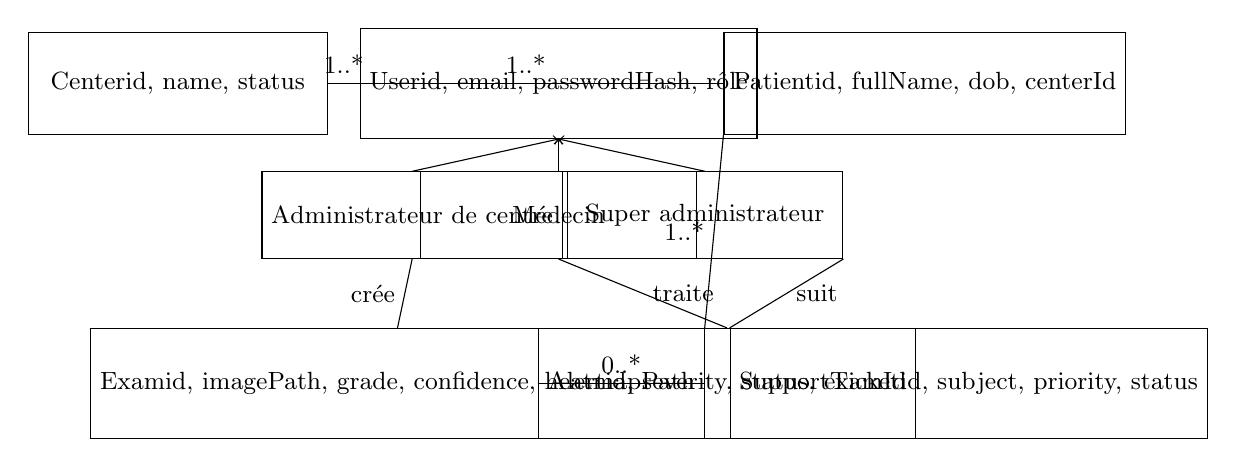
\begin{tikzpicture}[scale=0.93, every node/.style={font=\small}]
    % Classes principales
    \node[draw, rectangle, minimum width=3.8cm, minimum height=1.3cm] (center) at (2.0,7.0) {Center\\id, name, status};
    \node[draw, rectangle, minimum width=3.8cm, minimum height=1.4cm] (user) at (7.2,7.0) {User\\id, email, passwordHash, rôle};
    \node[draw, rectangle, minimum width=3.8cm, minimum height=1.3cm] (patient) at (12.2,7.0) {Patient\\id, fullName, dob, centerId};

    \node[draw, rectangle, minimum width=3.5cm, minimum height=1.1cm] (ca) at (5.2,5.2) {Administrateur de centre};
    \node[draw, rectangle, minimum width=3.5cm, minimum height=1.1cm] (doc) at (7.2,5.2) {Médecin};
    \node[draw, rectangle, minimum width=3.5cm, minimum height=1.1cm] (sa) at (9.2,5.2) {Super administrateur};

    \node[draw, rectangle, minimum width=4.0cm, minimum height=1.4cm] (exam) at (5.0,2.9) {Exam\\id, imagePath, grade, confidence, heatmapPath};
    \node[draw, rectangle, minimum width=4.0cm, minimum height=1.4cm] (alert) at (9.5,2.9) {Alert\\id, severity, status, examId};
    \node[draw, rectangle, minimum width=4.3cm, minimum height=1.4cm] (ticket) at (12.8,2.9) {SupportTicket\\id, subject, priority, status};

    % Relations
    \draw (center.east) -- node[above] {1..*} (user.west);
    \draw (center.east) -- node[above] {1..*} (patient.west);

    % Generalisation
    \draw[->] (ca.north) -- (user.south);
    \draw[->] (doc.north) -- (user.south);
    \draw[->] (sa.north) -- (user.south);

    \draw (patient.south west) -- node[left] {1..*} (exam.north east);
    \draw (ca.south) -- node[left] {crée} (exam.north);
    \draw (doc.south) -- node[right] {traite} (alert.north);
    \draw (exam.east) -- node[above] {0..*} (alert.west);
    \draw (sa.south east) -- node[right] {suit} (ticket.north west);
\end{tikzpicture}
\caption{Diagramme de classes general de la plateforme.}
\label{fig:class_general_ch2}
\end{figure}

\section{Architecture complète du système}

\subsection{Architecture du système (schéma global)}
Le schema global presente les couches logiques principales et les flux inter-services.

\begin{figure}[H]
\centering
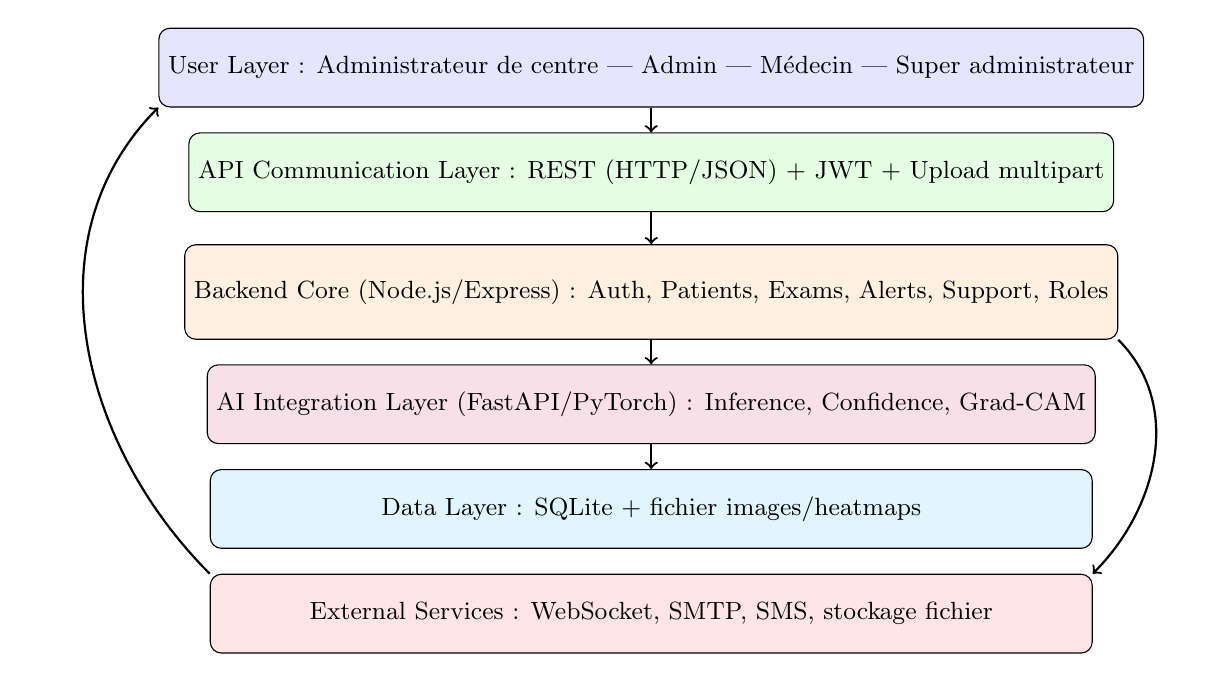
\begin{tikzpicture}[scale=0.95, every node/.style={font=\small}]
    \node[draw, rounded corners, fill=blue!10, minimum width=11.2cm, minimum height=1.0cm] (u) at (7.0,8.0) {User Layer : Administrateur de centre | Admin | Médecin | Super administrateur};
    \node[draw, rounded corners, fill=green!10, minimum width=11.2cm, minimum height=1.0cm] (api) at (7.0,6.6) {API Communication Layer : REST (HTTP/JSON) + JWT + Upload multipart};
    \node[draw, rounded corners, fill=orange!12, minimum width=11.2cm, minimum height=1.2cm] (core) at (7.0,5.0) {Backend Core (Node.js/Express) : Auth, Patients, Exams, Alerts, Support, Roles};
    \node[draw, rounded corners, fill=purple!12, minimum width=11.2cm, minimum height=1.0cm] (ai) at (7.0,3.5) {AI Integration Layer (FastAPI/PyTorch) : Inference, Confidence, Grad-CAM};
    \node[draw, rounded corners, fill=cyan!12, minimum width=11.2cm, minimum height=1.0cm] (data) at (7.0,2.1) {Data Layer : SQLite + fichier images/heatmaps};
    \node[draw, rounded corners, fill=red!10, minimum width=11.2cm, minimum height=1.0cm] (ext) at (7.0,0.7) {External Services : WebSocket, SMTP, SMS, stockage fichier};

    \draw[->, thick] (u.south) -- (api.north);
    \draw[->, thick] (api.south) -- (core.north);
    \draw[->, thick] (core.south) -- (ai.north);
    \draw[->, thick] (ai.south) -- (data.north);
    \draw[->, thick] (core.south east) to[out=-45,in=45] (ext.north east);
    \draw[->, thick] (ext.north west) to[out=135,in=-135] (u.south west);
\end{tikzpicture}
\caption{Schéma global de l'architecture du système.}
\label{fig:archi_globale_ch2}
\end{figure}

\subsection{Architecture globale de la plateforme}
L'architecture globale du système suit un enchaînement simple et lisible : les utilisateurs accèdent à l'interface web, les requêtes passent par l'API du backend, le service IA traite les images rétiniennes, puis les données et résultats sont stockés et diffusés aux différents rôles.

\begin{figure}[H]
\centering
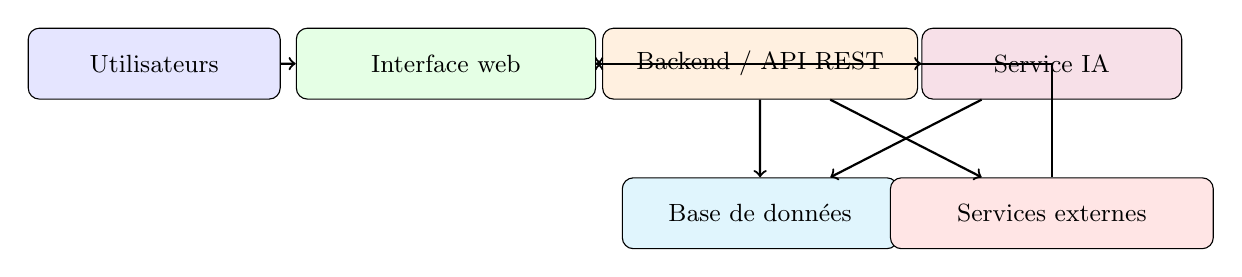
\begin{tikzpicture}[scale=0.95, every node/.style={font=\small}]
    \node[draw, rounded corners, fill=blue!10, minimum width=3.2cm, minimum height=0.9cm] (user) at (1.8,4.0) {Utilisateurs};
    \node[draw, rounded corners, fill=green!10, minimum width=3.8cm, minimum height=0.9cm] (front) at (5.7,4.0) {Interface web};
    \node[draw, rounded corners, fill=orange!12, minimum width=4.0cm, minimum height=0.9cm] (back) at (9.9,4.0) {Backend / API REST};
    \node[draw, rounded corners, fill=purple!12, minimum width=3.3cm, minimum height=0.9cm] (ai) at (13.8,4.0) {Service IA};

    \node[draw, rounded corners, fill=cyan!12, minimum width=3.5cm, minimum height=0.9cm] (data) at (9.9,2.0) {Base de données};
    \node[draw, rounded corners, fill=red!10, minimum width=4.1cm, minimum height=0.9cm] (ext) at (13.8,2.0) {Services externes};

    \draw[->, thick] (user) -- (front);
    \draw[->, thick] (front) -- (back);
    \draw[->, thick] (back) -- (ai);
    \draw[->, thick] (back) -- (data);
    \draw[->, thick] (back) -- (ext);
    \draw[->, thick] (ai) -- (data);
    \draw[->, thick] (ext) |- (front);
\end{tikzpicture}
\caption{Schéma global simplifié de l'architecture du système.}
\label{fig:archi_globale_simple_ch2}
\end{figure}

\noindent
Les elements principaux sont :
\begin{itemize}
    \item \textbf{Interface web} : accès des différents rôles au système ;
    \item \textbf{Backend / API} : gestion des règles métier et de la sécurité ;
    \item \textbf{Service IA} : analyse des images retiniennes et production des resultats ;
    \item \textbf{Base de données} : stockage des comptes, patients, examens et alertes ;
    \item \textbf{Services externes} : notifications et communication temps reel.
\end{itemize}

\subsection{Architecture detaillee (diagrammes de sequence)}
Les diagrammes suivants decrivent les echanges applicatifs sur des scenarios critiques,
avec un accent sur la responsabilité clinique, la traçabilité et la priorisation des cas à risque.

\subsubsection*{Authentification sécurisée et responsabilité clinique}
\begin{figure}[H]
        \centering
        \includegraphics[width=1\\linewidth]{nchlh auth final.png}
    \caption{Diagramme de séquence - Authentification sécurisée et traçabilité d'accès}
\end{figure}
Ce diagramme détaille le contrôle d'accès par rôle, la création de session JWT et la traçabilité des connexions pour sécuriser les actions cliniques et administratives.

\subsubsection*{Création d'examen et orchestration clinique}
\begin{figure}[H]
    \centering
            \includegraphics[width=1\linewidth]{oyaaaaaaaaa.png}
    \caption{Diagramme de séquence - Création d'examen par l'Administrateur de centre}
\end{figure}
Ce diagramme illustre la création d'un examen médical, l'envoi de l'image rétinienne et l'orchestration du flux clinique jusqu'au déclenchement de l'analyse IA.

\subsubsection*{Analyse IA, triage clinique et generation d'alerte}
\begin{figure}[H]
               \centering
               \includegraphics[width=1\linewidth]{zab.pdf4.png}
    \caption{Diagramme de sequence - Analyse IA et priorisation des alertes cliniques}
\end{figure}
Ce diagramme présente l'inférence IA, la production de l'explicabilité (Grad-CAM) et la création d'alertes pour orienter rapidement les cas sévères vers le médecin.

\subsubsection*{Création de centre et attribution d'administration}
\begin{figure}[H]
         \centering
     \includegraphics[width=1\linewidth]{nchlh superfinal.png}
    \caption{Diagramme de séquence - Création de centre et attribution de l'administrateur de centre}
\end{figure}
Ce diagramme décrit la gouvernance plateforme assurée par le Super administrateur : création/configuration de centre, attribution des droits et continuités des opérations cliniques.

\subsection{Hardware environment}
L'environnement materiel requis est defini a deux niveaux.

\subsubsection*{Machine de developpement}
\begin{itemize}
    \item système Windows ou Linux ;
    \item processeur multi-coeurs (classe Intel Core i5/i7 ou equivalent) ;
    \item memoire RAM recommandee : 16 Go ou plus ;
    \item stockage SSD pour accélérer les accès aux datasets/modèles.
\end{itemize}

\subsubsection*{Machine d'execution IA}
\begin{itemize}
    \item CPU moderne pour inference standard ;
    \item GPU optionnel (CUDA) pour acceleration de l'inference et des batchs ;
    \item espace disque suffisant pour modeles, checkpoints et heatmaps.
\end{itemize}

\subsection{Software environment}

\subsubsection*{Development tools}
\begin{itemize}
    \item Visual Studio Code ;
    \item Git/GitHub pour le versioning ;
    \item Postman (ou equivalent) pour tests API ;
    \item scripts Python/Node pour automatisation des taches techniques.
\end{itemize}

\subsubsection*{Frontend environment (framework, design, API communication)}
\begin{itemize}
    \item frontend web en HTML/CSS/JavaScript ;
    \item design responsive pour dashboards Administrateur de centre/Médecin/Super administrateur ;
    \item consommation API backend via requetes HTTP ;
    \item reception des evenements temps reel via WebSocket.
\end{itemize}

\subsubsection*{Backend environment (framework, language, architecture, API type)}
\begin{itemize}
    \item langage : JavaScript (Node.js) ;
    \item framework : Express.js ;
    \item architecture backend modulaire (routes, middleware, services, config) ;
    \item API de type REST sécurisée par JWT.
\end{itemize}

\subsubsection*{AI service environment}
\begin{itemize}
    \item langage : Python ;
    \item framework API : FastAPI ;
    \item bibliotheques IA : PyTorch, TorchVision, OpenCV, Pillow, NumPy ;
    \item execution modele + production heatmap via endpoints dedies.
\end{itemize}

\subsubsection*{Data storage}
\begin{itemize}
    \item base relationnelle legere : SQLite ;
    \item organisation des fichiers images/resultats dans des repertoires structures ;
    \item sauvegarde périodique recommandée pour données critiques.
\end{itemize}

\subsubsection*{Realtime communication}
\begin{itemize}
    \item service WebSocket pour notifications instantanees ;
    \item diffusion sélective des événements selon le rôle ;
    \item synchronisation des dashboards avec l'etat des examens/alertes.
\end{itemize}

\section{Fiches descriptives des cas d'utilisation}
Les fiches suivantes presentent de maniere detaillee et homogeneisee chaque cas d'utilisation principal,
en utilisant une structure coherente : objectif, acteurs, preconditions, scenarios et postconditions.

\subsection{Cas d'utilisation - Administrateur de centre : Orchestration opérationnelle du dépistage clinique}
\begin{table}[H]
\centering
\renewcommand{\arraystretch}{1.3}
\begin{tabular}{|p{5cm}|p{10cm}|}
\hline
\textbf{Nom du cas d'utilisation} & Orchestration opérationnelle du dépistage clinique \\ \hline

\textbf{Objectif} & Permettre à l'Administrateur de centre d'orchestrer les flux de dépistage clinique, de garantir la qualité des données et d'assurer le suivi des demandes de support opérationnel en vue d'optimiser la prise en charge clinique. \\ \hline

\textbf{Acteur principal} & Administrateur de centre \\ \hline

\textbf{Préconditions} & 
\begin{itemize}
\item Administrateur de centre authentifié et connecté au système.
\item Centre actif et accessible.
\end{itemize} \\ \hline

\textbf{Scénario nominal} & 
\begin{itemize}
\item L'Administrateur de centre accede au tableau de bord du centre.
\item Il consulte les dossiers en attente et priorise les examens a demarrer.
\item Il selectionne ou ajoute un patient si necessaire.
\item Il démarre l'examen (création, paramètres et téléversement d'image rétinienne si capture externe).
\item Le système enregistre l'examen et déclenche l'analyse IA automatiquement.
\item L'Administrateur de centre consulte l'etat de l'examen et les resultats IA.
\item Si nécessaire, il accède à la section support et crée une demande d'assistance.
\item Il suit l'etat de la demande de support.
\end{itemize} \\\hline

\textbf{Scénarios alternatifs} &
\begin{itemize}
\item Erreur lors du téléversement de l'image (format invalide, fichier corrompu).
\item Données patient incomplètes (nom, date de naissance manquants).
\item Médecin non disponible au centre.
\item Ticket support non traite ou en attente de reponse prolongee.
\end{itemize} \\ \hline

\textbf{Postconditions} & 
\begin{itemize}
\item L'examen est enregistré dans le système.
\item La demande de support est créée ou mise à jour.
\item L'analyse IA est declenchee ou comfortee.
\end{itemize} \\ \hline
\end{tabular}
\caption{Fiche descriptive - Administrateur de centre (orchestration opérationnelle du dépistage clinique)}
\end{table}

\subsection{Cas d'utilisation - Médecin : Validation diagnostique et prise de décision clinique}
\begin{table}[H]
\centering
\renewcommand{\arraystretch}{1.3}
\begin{tabular}{|p{5cm}|p{10cm}|}
\hline
\textbf{Nom du cas d'utilisation} & Validation diagnostique et prise de décision clinique \\ \hline

\textbf{Objectif} & Permettre au Médecin de valider les prédictions IA, d'interpréter rigoureusement les données cliniques et de prendre une décision thérapeutique éclairée et responsable pour assurer la qualité des soins. \\ \hline

\textbf{Acteur principal} & Médecin \\ \hline

\textbf{Preconditions} & 
\begin{itemize}
\item Médecin authentifié et connecté au système.
\item Examens disponibles et analyses par le service IA.
\end{itemize} \\ \hline

\textbf{Scenario nominal} &
\begin{itemize}
\item Le Médecin se connecte au système et accède au tableau de bord.
\item Le système affiche en priorité les cas sévères (alertes avec grade $\geq 3$).
\item Le Médecin consulte les examens urgents en premier.
\item Il visualise l'image retinienne originale associee a l'examen.
\item Il examine la prediction IA (grade, score de confiance) et la heatmap Grad-CAM.
\item Le Médecin analyse le cas et prend une décision clinique.
\item Il redige le rapport d'examen avec son interpretation clinique.
\item Il consulte l'historique des examens du patient pour suivi longitudinal.
\item Il marque l'alerte comme traitée dans le système.
\item Il télécharge l'examen complet pour archivage ou impression si nécessaire.
\end{itemize} \\ \hline

\textbf{Scenarios alternatifs} &
\begin{itemize}
\item Pas d'images retiniennes disponibles pour consultation.
\item Le modele IA n'a pu generer de prediction (image corrompue ou invalide).
\item Heatmap indisponible ou de mauvaise qualité.
\item Données patient incomplètes ou incohérentes.
\item Alerte déjà traitée par un autre médecin.
\end{itemize} \\ \hline

\textbf{Postconditions} &
\begin{itemize}
\item L'examen est consulte et interprete.
\item Le rapport clinique est redige et enregistre.
\item L'alerte est marquee comme resolue ou redirigee.
\item L'historique du patient est disponible pour suivi.
\end{itemize} \\ \hline
\end{tabular}
\caption{Fiche descriptive - Médecin (validation diagnostique et prise de décision clinique)}
\end{table}

\subsection{Cas d'utilisation - Super administrateur : Pilotage stratégique et supervision clinique globale}
\begin{table}[H]
\centering
\renewcommand{\arraystretch}{1.3}
\begin{tabular}{|p{5cm}|p{10cm}|}
\hline
\textbf{Nom du cas d'utilisation} & Pilotage strategique et supervision clinique globale \\ \hline

\textbf{Objectif} & Assurer la gouvernance globale de la plateforme, superviser les indicateurs cliniques, suivre les centres actifs et garantir la disponibilité ainsi que la fiabilité du système au service de l'excellence médicale. \\ \hline

\textbf{Acteur principal} & Super administrateur \\ \hline

\textbf{Preconditions} &
\begin{itemize}
\item Super administrateur authentifié et connecté au système.
\item Droits d'administration globale confirmes.
\end{itemize} \\ \hline

\textbf{Scenario nominal} &
\begin{itemize}
\item Le Super administrateur accede au tableau de bord global de la plateforme.
\item Il gère la création, la configuration, l'activation et la suspension/désactivation des centres.
\item Il attribue ou retire le statut d'administrateur de centre aux utilisateurs concernes.
\item Il centralise et suit les incidents et demandes d'assistance provenant de tous les centres.
    \item Il priorise les tickets et coordonne leur traitement avec les équipes de support.
    \item Il vérifie la disponibilité et la performance des services critiques (backend, IA, base de données).
\item Il documente les actions et décisions prises pour assurer la traçabilité.
\item Ce rôle est global, distinct d'un administrateur de centre, et pourra évoluer avec de nouvelles responsabilités.
\end{itemize} \\ \hline

\textbf{Scenarios alternatifs} &
\begin{itemize}
\item Un centre ne repond plus (indisponibilite du service).
\item Nombreuses erreurs IA detectees pour une region specifique.
\item Anomalie de performance : ralentissement général du système.
\item Utilisateur avec droits incorrects ou suspects.
\item Stockage disque saturation approchant la limite critique.
\end{itemize} \\ \hline

\textbf{Postconditions} &
\begin{itemize}
\item Les centres sont mis a jour et administres.
\item Les utilisateurs et leurs droits sont valides.
\item Les alertes système sont résolues ou escaladées.
\item Les statistiques et metriques sont documentees.
\end{itemize} \\ \hline
\end{tabular}
\caption{Fiche descriptive - Super administrateur (pilotage stratégique et supervision clinique globale)}
\end{table}

\subsection{Cas d'utilisation - Service IA : Support décisionnel et traçabilité diagnostique}
\begin{table}[H]
\centering
\renewcommand{\arraystretch}{1.3}
\begin{tabular}{|p{5cm}|p{10cm}|}
\hline
\textbf{Nom du cas d'utilisation} & Support décisionnel et traçabilité diagnostique \\ \hline

\textbf{Objectif} & Fournir une analyse automatisée rigoureuse des images rétiniennes, générer des prédictions cliniquement pertinentes avec confiance quantifiée et produire des explications visuelles (Grad-CAM) pour soutenir la décision diagnostique du médecin. \\ \hline

\textbf{Acteur principal} & Service IA (FastAPI + ResNet) \\ \hline

\textbf{Preconditions} &
\begin{itemize}
\item Une image retinienne valide  est disponible.
\item L'examen a été créé dans le système et authentifié.
\item Le modele ResNet est charge et operationnel.
\item Ressources de calcul (CPU/GPU) sont disponibles.
\end{itemize} \\ \hline

\textbf{Scenario nominal} &
\begin{itemize}
\item Le backend envoie l'image retinienne au Service IA via appel HTTP.
\item Le Service IA receptionne l'image et valide son format.
\item L'image est pretraitee (normalisation, redimensionnement, augmentation si necessaire).
\item Le modele ResNet effectue l'inference sur l'image pretraitee.
\item Le système prédit le grade de rétinopathie (0, 1, 2, 3 ou 4).
\item Le score de confiance (probabilite) est calcule a partir des logits.
\item Une heatmap Grad-CAM est générée pour expliquer la décision du modèle.
\item Les resultats (grade, confiance, chemin de la heatmap) sont retournes au backend en format JSON.
\item Le backend enregistre les résultats dans la base de données.
\item Les resultats sont rendus disponibles a l'interface Médecin pour consultation.
\end{itemize} \\ \hline

\textbf{Scenarios alternatifs} &
\begin{itemize}
\item Image invalide ou corrompue : rejet avec message d'erreur.
\item Format d'image non supporte : conversion ou rejet.
\item Echec du modele IA (poids manquants, memoire insuffisante) : erreur HTTP 500.
\item Temps de reponse trop eleve (>30 secondes) : timeout possible du frontend.
\item Heatmap non generee pour raison technique : resultat IA retourne sans heatmap.
\end{itemize} \\ \hline

\textbf{Postconditions} &
\begin{itemize}
\item Les resultats de prediction (grade, confiance, heatmap) sont generes et stockes.
\item Les données sont accessibles pour consultation par le médecin.
\item Un enregistrement de trace (logs) est conserve pour audit et debugging.
\end{itemize} \\ \hline
\end{tabular}
\caption{Fiche descriptive - Service IA (support décisionnel et traçabilité diagnostique)}
\end{table}

\subsection{Cas d'utilisation - Tous les acteurs : Authentification sécurisée et responsabilité clinique}
\begin{table}[H]
\centering
\renewcommand{\arraystretch}{1.3}
\begin{tabular}{|p{5cm}|p{10cm}|}
\hline
\textbf{Nom du cas d'utilisation} & Authentification sécurisée et responsabilité clinique \\ \hline

\textbf{Objectif} & Autoriser les utilisateurs cliniques et administratifs à s'authentifier de manière sécurisée, maintenir la traçabilité des actions dans un contexte réglementaire médicale et terminer leur session de manière fiable. \\ \hline

\textbf{Acteur principal} & Tous les acteurs (Administrateur de centre, Admin, Médecin, Super administrateur) \\ \hline

\textbf{Preconditions} &
\begin{itemize}
\item Compte utilisateur existe et est actif dans le système.
\item Centre affilie (le cas echeant) est actif.
\end{itemize} \\ \hline

\textbf{Scenario nominal} &
\begin{itemize}
\item L'utilisateur accede a la page de connexion.
\item Il saisit ses identifiants (email, mot de passe).
\item Le système valide les identifiants contre la base de données.
\item Le système génère un token JWT sécurisé et stocke la session.
\item L'utilisateur est redirigé vers le tableau de bord correspondant à son rôle.
\item L'utilisateur peut effectuer les actions autorisées par son rôle.
\item L'utilisateur clique sur deconnexion.
\item Le système invalide le token et termine la session.
\item L'utilisateur est redirige vers la page de connexion.
\end{itemize} \\ \hline

\textbf{Scenarios alternatifs} &
\begin{itemize}
\item Identifiants incorrects : message d'erreur et tentative d'authentification.
\item Compte désactivé ou supprimé : refus d'accès.
\item Centre affilié non actif : refus d'accès pour Administrateur de centre/Médecin.
\item Session expieree apres inactivite prolongee : redirection a la connexion.
\item Token invalide ou manipulé : refus d'accès et redirection à la connexion.
\end{itemize} \\ \hline

\textbf{Postconditions} &
\begin{itemize}
\item Utilisateur authentifié et session créée OU utilisateur déconnecté et session terminée.
\item Droits d'accès basés sur le rôle sont appliqués.
\end{itemize} \\ \hline
\end{tabular}
\caption{Fiche descriptive - Authentification et gestion de session}
\end{table}

\section{Conclusion}
Ce chapitre a présenté une spécification complète du système, depuis l'analyse des acteurs
jusqu'a l'architecture technique detaillee. La modelisation proposee garantit une base coherente
pour l'implementation et la validation de la plateforme en contexte reel.

Les fiches descriptives des cas d'utilisation offrent une formalisation rigoureuse et homogeneisee,
facilitant la communication entre les équipes métier, de conception et de développement.

La suite du rapport peut s'appuyer sur ce cadre pour decrire la realisation,
les tests d'integration et l'evaluation finale de la solution.
% =========================

\chapter{Analyse du système et architecture technique}
\label{chap:analyse_architecture}

\section{Introduction}
Ce chapitre formalise la vision système de la plateforme de dépistage automatisé de la rétinopathie diabétique.
Il présente d'abord l'analyse du système (acteurs, exigences), puis la modélisation UML globale,
et enfin l'architecture complete de la solution (logicielle, materielle et operationnelle).

Le contenu est appliqué au projet réalisé, en conservant les rôles métier réels :
\textbf{Administrateur de centre}, \textbf{Admin}, \textbf{Médecin}, \textbf{Super administrateur}, ainsi que l'acteur technique secondaire \textbf{Service IA}.

\section{Analyse du système}

\subsection{Acteurs}
Les acteurs identifiés sont classés en deux catégories : acteurs humains (métier) et acteurs système (techniques).

\subsubsection*{Acteurs humains (Human Actors)}
\begin{itemize}
    \item \textbf{Administrateur de centre} : gère les patients et les médecins du centre, crée les examens,
    envoie les images rétiniennes et consulte l'historique.
    \item \textbf{Admin} : assure l'administration applicative courante (parametrage, suivi operationnel,
    controle des utilisateurs selon les droits attribues).
    \item \textbf{Médecin} : consulte les examens classes par priorite, interprete la prediction IA et la heatmap,
    puis valide la conduite clinique.
    \item \textbf{Super administrateur} : administre les centres, gère la gouvernance globale (comptes, support, supervision,
    disponibilité du système).
\end{itemize}

\subsubsection*{Acteurs système (System Actors)}
\begin{itemize}
    \item \textbf{Service IA} (acteur secondaire principal) : reçoit l'image, exécute l'inférence,
    génère la heatmap Grad-CAM et retourne grade + confiance.
    \item \textbf{Service WebSocket} : diffuse les notifications temps reel (nouveaux examens, alertes severes,
    mises a jour d'etat).
    \item \textbf{Serveur SMTP/SMS} : assure les communications asynchrones (notifications, alertes critiques).
\end{itemize}

\textbf{Note de modelisation :} \textit{Patient} et \textit{Center} ne sont pas des acteurs,
mais des entités métier manipulées par les acteurs humains.

\subsection{Exigences fonctionnelles}
Les exigences fonctionnelles du système sont regroupées par domaine métier.

\subsubsection*{Gestion des comptes et sécurité}
\begin{itemize}
    \item authentification par rôle (Administrateur de centre, Admin, Médecin, Super administrateur) ;
    \item autorisation basée sur le rôle pour chaque route métier ;
    \item gestion de session et deconnexion sécurisée.
\end{itemize}

\subsubsection*{Gestion operationnelle du depistage}
\begin{itemize}
    \item création/modification/consultation/archivage de patients ;
    \item gestion des médecins rattachés à un centre ;
    \item création d'un examen avec téléversement d'image rétinienne ;
    \item association patient-médecin-centre lors de la création d'examen.
\end{itemize}

\subsubsection*{Analyse IA et explicabilité}
\begin{itemize}
    \item envoi de l'image vers le service IA ;
    \item prédiction automatique du grade de rétinopathie (0 à 4) ;
    \item calcul du score de confiance ;
    \item génération et stockage d'une heatmap Grad-CAM ;
    \item restitution du résultat dans l'interface Médecin.
\end{itemize}

\subsubsection*{Alertes et supervision}
\begin{itemize}
    \item création automatique d'alerte pour les cas sévères (grade $\geq 3$) ;
    \item notification temps réel du Médecin ;
    \item suivi de l'état des alertes (nouvelle, en cours, résolue) ;
    \item supervision transversale des centres et du support par le Super administrateur.
\end{itemize}

\subsection{Exigences non fonctionnelles}
Les exigences non fonctionnelles assurent la qualité globale du système en production.

\begin{itemize}
    \item \textbf{Performance} : temps de reponse court pour l'inference et l'affichage ;
    \item \textbf{Disponibilité} : accès continu des interfaces centre, médecin et supervision ;
    \item \textbf{Sécurité} : protection des données médicales, contrôle d'accès et isolation par centre ;
    \item \textbf{Fiabilité} : traçabilité des examens, alertes et actions utilisateurs ;
    \item \textbf{Scalabilite} : possibilite d'augmenter le nombre de centres et le volume d'images ;
    \item \textbf{Maintenabilite} : architecture modulaire (frontend, backend, IA, realtime) ;
    \item \textbf{Explicabilité} : visualisation interprétable (Grad-CAM) pour appuyer la décision clinique.
\end{itemize}

\section{Modélisation du système}

\subsection{Diagramme de cas d'utilisation général}
Le diagramme suivant represente la vue fonctionnelle globale avec
quatre acteurs primaires (Administrateur de centre, Admin, Médecin, Super administrateur) et un acteur secondaire (Service IA).

\begin{figure}[H]
\centering
\begin{tikzpicture}[scale=0.86, every node/.style={font=\small}]
    % Limite système
    \draw[thick] (1.8,0.6) rectangle (13.0,8.4);
    \node[anchor=west] at (2.0,8.1) {Système de dépistage RD};

    % Acteurs gauche
    % Administrateur de centre
    \draw (0.3,6.7) circle (0.25);
    \draw (0.3,6.45) -- (0.3,5.7);
    \draw (-0.2,6.05) -- (0.8,6.05);
    \draw (0.3,5.7) -- (-0.05,5.1);
    \draw (0.3,5.7) -- (0.65,5.1);
    \node at (0.3,4.8) {Administrateur de centre};

    % Admin
    \draw (-1.0,4.8) circle (0.25);
    \draw (-1.0,4.55) -- (-1.0,3.8);
    \draw (-1.5,4.15) -- (-0.5,4.15);
    \draw (-1.0,3.8) -- (-1.35,3.2);
    \draw (-1.0,3.8) -- (-0.65,3.2);
    \node at (-1.0,2.9) {Admin};

    % Médecin
    \draw (0.3,4.2) circle (0.25);
    \draw (0.3,3.95) -- (0.3,3.2);
    \draw (-0.2,3.55) -- (0.8,3.55);
    \draw (0.3,3.2) -- (-0.05,2.6);
    \draw (0.3,3.2) -- (0.65,2.6);
    \node at (0.3,2.3) {Médecin};

    % Super administrateur
    \draw (0.3,1.8) circle (0.25);
    \draw (0.3,1.55) -- (0.3,0.8);
    \draw (-0.2,1.15) -- (0.8,1.15);
    \draw (0.3,0.8) -- (-0.05,0.25);
    \draw (0.3,0.8) -- (0.65,0.25);
    \node at (0.3,-0.05) {Super administrateur};

    % Acteur secondaire droite : Service IA
    \draw (14.4,4.4) circle (0.25);
    \draw (14.4,4.15) -- (14.4,3.4);
    \draw (13.9,3.8) -- (14.9,3.8);
    \draw (14.4,3.4) -- (14.05,2.8);
    \draw (14.4,3.4) -- (14.75,2.8);
    \node at (14.4,2.45) {Service IA};

    % Use cases
    \node[draw, ellipse, minimum width=4.7cm, minimum height=0.85cm] (u1) at (5.5,7.3) {Se connecter};
    \node[draw, ellipse, minimum width=4.7cm, minimum height=0.85cm] (u2) at (5.5,6.2) {Gérer patients};
    \node[draw, ellipse, minimum width=4.7cm, minimum height=0.85cm] (u3) at (5.5,5.1) {Gérer médecins};
    \node[draw, ellipse, minimum width=4.7cm, minimum height=0.85cm] (u4) at (5.5,4.0) {Créer examen};
    \node[draw, ellipse, minimum width=4.7cm, minimum height=0.85cm] (u5) at (5.5,2.9) {Consulter historique};
    \node[draw, ellipse, minimum width=4.7cm, minimum height=0.85cm] (u6) at (9.4,5.8) {Consulter examens et alertes};
    \node[draw, ellipse, minimum width=4.7cm, minimum height=0.85cm] (u7) at (9.4,4.5) {Interpreter prediction + heatmap};
    \node[draw, ellipse, minimum width=4.7cm, minimum height=0.85cm] (u8) at (9.4,3.2) {Superviser centres et support};
    \node[draw, ellipse, minimum width=4.7cm, minimum height=0.85cm] (u9) at (9.4,1.9) {Administrer comptes globaux};
    \node[draw, ellipse, minimum width=4.7cm, minimum height=0.85cm] (u10) at (7.5,0.95) {Se déconnecter};
    \node[draw, ellipse, minimum width=4.7cm, minimum height=0.85cm] (u11) at (11.0,6.95) {Analyser image rétinienne};

    % Liens Administrateur de centre
    \draw (0.8,6.05) -- (u1.west);
    \draw (0.8,6.05) -- (u2.west);
    \draw (0.8,6.05) -- (u3.west);
    \draw (0.8,6.05) -- (u4.west);
    \draw (0.8,6.05) -- (u5.west);
    \draw (0.8,6.05) -- (u10.west);

    % Liens Médecin
    \draw (0.8,3.55) -- (u1.west);
    \draw (0.8,3.55) -- (u6.west);
    \draw (0.8,3.55) -- (u7.west);
    \draw (0.8,3.55) -- (u10.west);

    % Liens Admin
    \draw (-0.5,4.15) -- (u1.west);
    \draw (-0.5,4.15) -- (u2.west);
    \draw (-0.5,4.15) -- (u3.west);
    \draw (-0.5,4.15) -- (u5.west);
    \draw (-0.5,4.15) -- (u10.west);

    % Liens Super administrateur
    \draw (0.8,1.15) -- (u1.west);
    \draw (0.8,1.15) -- (u8.west);
    \draw (0.8,1.15) -- (u9.west);
    \draw (0.8,1.15) -- (u10.west);

    % Include vers IA
    \draw[->, dashed] (u4.east) -- (u11.west);
    \node at (8.6,6.6) {<<include>>};
    \draw[->, dashed] (u7.north) -- (u11.south);
    \node at (10.3,5.9) {<<include>>};

    % Lien acteur IA
    \draw (13.9,3.8) -- (u11.east);
\end{tikzpicture}
\caption{Diagramme de cas d'utilisation général du système.}
\label{fig:usecase_general_ch2}
\end{figure}

\subsection{Diagramme de classes general}
Le diagramme de classes ci-dessous montre les principales entités métier,
les specialisations de l'utilisateur et les relations entre objets applicatifs

\begin{figure}[H]
\centering
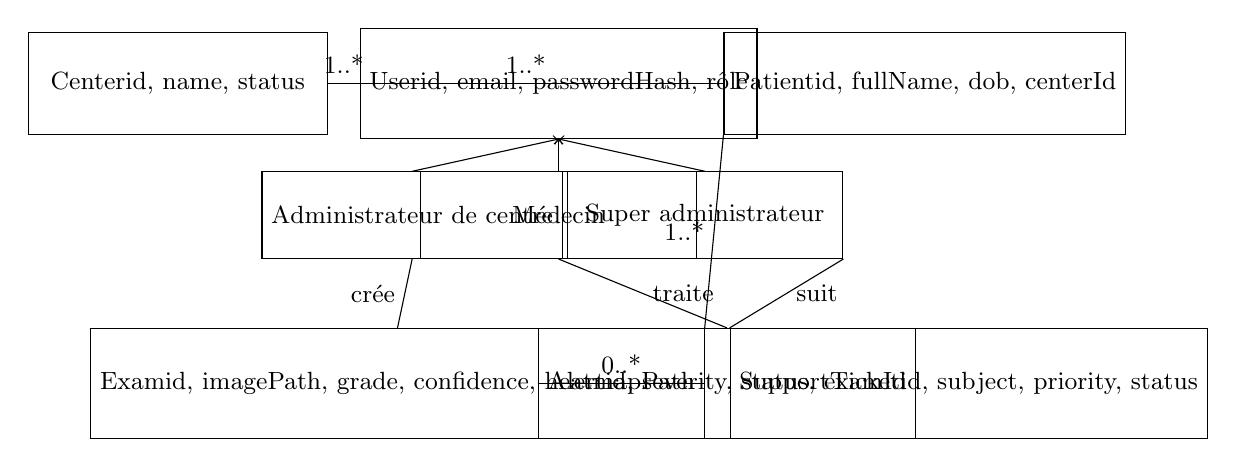
\begin{tikzpicture}[scale=0.93, every node/.style={font=\small}]
    % Classes principales
    \node[draw, rectangle, minimum width=3.8cm, minimum height=1.3cm] (center) at (2.0,7.0) {Center\\id, name, status};
    \node[draw, rectangle, minimum width=3.8cm, minimum height=1.4cm] (user) at (7.2,7.0) {User\\id, email, passwordHash, rôle};
    \node[draw, rectangle, minimum width=3.8cm, minimum height=1.3cm] (patient) at (12.2,7.0) {Patient\\id, fullName, dob, centerId};

    \node[draw, rectangle, minimum width=3.5cm, minimum height=1.1cm] (ca) at (5.2,5.2) {Administrateur de centre};
    \node[draw, rectangle, minimum width=3.5cm, minimum height=1.1cm] (doc) at (7.2,5.2) {Médecin};
    \node[draw, rectangle, minimum width=3.5cm, minimum height=1.1cm] (sa) at (9.2,5.2) {Super administrateur};

    \node[draw, rectangle, minimum width=4.0cm, minimum height=1.4cm] (exam) at (5.0,2.9) {Exam\\id, imagePath, grade, confidence, heatmapPath};
    \node[draw, rectangle, minimum width=4.0cm, minimum height=1.4cm] (alert) at (9.5,2.9) {Alert\\id, severity, status, examId};
    \node[draw, rectangle, minimum width=4.3cm, minimum height=1.4cm] (ticket) at (12.8,2.9) {SupportTicket\\id, subject, priority, status};

    % Relations
    \draw (center.east) -- node[above] {1..*} (user.west);
    \draw (center.east) -- node[above] {1..*} (patient.west);

    % Generalisation
    \draw[->] (ca.north) -- (user.south);
    \draw[->] (doc.north) -- (user.south);
    \draw[->] (sa.north) -- (user.south);

    \draw (patient.south west) -- node[left] {1..*} (exam.north east);
    \draw (ca.south) -- node[left] {crée} (exam.north);
    \draw (doc.south) -- node[right] {traite} (alert.north);
    \draw (exam.east) -- node[above] {0..*} (alert.west);
    \draw (sa.south east) -- node[right] {suit} (ticket.north west);
\end{tikzpicture}
\caption{Diagramme de classes general de la plateforme.}
\label{fig:class_general_ch2}
\end{figure}

\section{Architecture complète du système}

\subsection{Architecture du système (schéma global)}
Le schema global presente les couches logiques principales et les flux inter-services.

\begin{figure}[H]
\centering
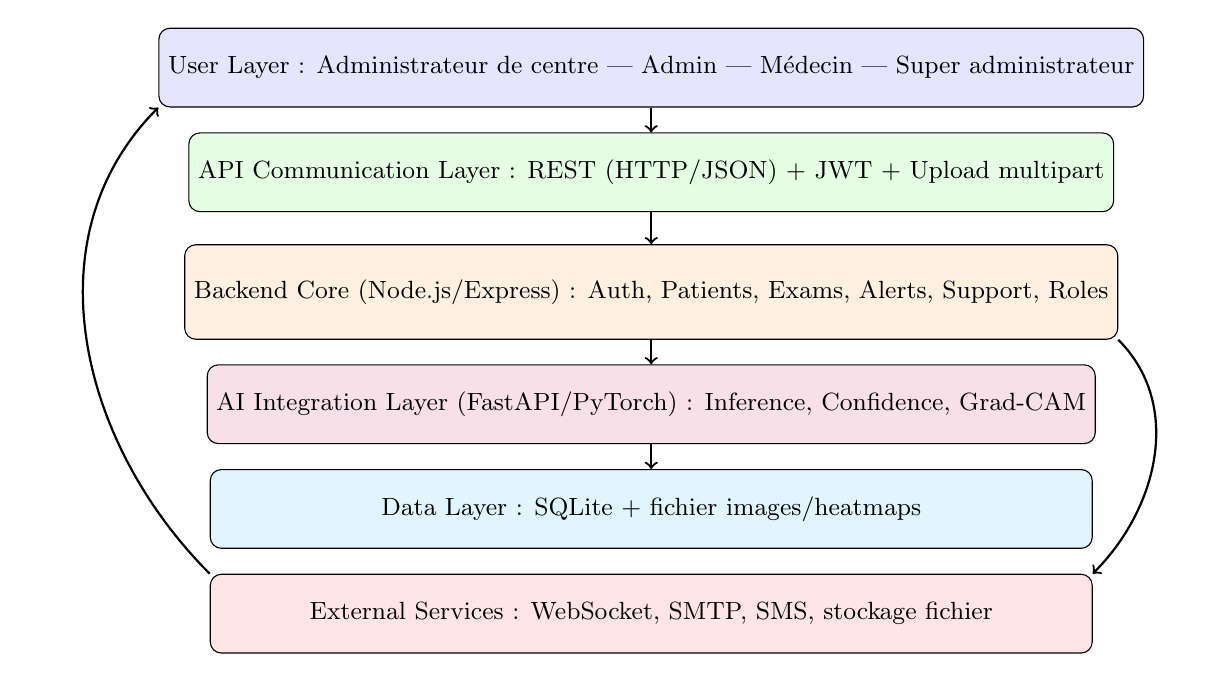
\begin{tikzpicture}[scale=0.95, every node/.style={font=\small}]
    \node[draw, rounded corners, fill=blue!10, minimum width=11.2cm, minimum height=1.0cm] (u) at (7.0,8.0) {User Layer : Administrateur de centre | Admin | Médecin | Super administrateur};
    \node[draw, rounded corners, fill=green!10, minimum width=11.2cm, minimum height=1.0cm] (api) at (7.0,6.6) {API Communication Layer : REST (HTTP/JSON) + JWT + Upload multipart};
    \node[draw, rounded corners, fill=orange!12, minimum width=11.2cm, minimum height=1.2cm] (core) at (7.0,5.0) {Backend Core (Node.js/Express) : Auth, Patients, Exams, Alerts, Support, Roles};
    \node[draw, rounded corners, fill=purple!12, minimum width=11.2cm, minimum height=1.0cm] (ai) at (7.0,3.5) {AI Integration Layer (FastAPI/PyTorch) : Inference, Confidence, Grad-CAM};
    \node[draw, rounded corners, fill=cyan!12, minimum width=11.2cm, minimum height=1.0cm] (data) at (7.0,2.1) {Data Layer : SQLite + fichier images/heatmaps};
    \node[draw, rounded corners, fill=red!10, minimum width=11.2cm, minimum height=1.0cm] (ext) at (7.0,0.7) {External Services : WebSocket, SMTP, SMS, stockage fichier};

    \draw[->, thick] (u.south) -- (api.north);
    \draw[->, thick] (api.south) -- (core.north);
    \draw[->, thick] (core.south) -- (ai.north);
    \draw[->, thick] (ai.south) -- (data.north);
    \draw[->, thick] (core.south east) to[out=-45,in=45] (ext.north east);
    \draw[->, thick] (ext.north west) to[out=135,in=-135] (u.south west);
\end{tikzpicture}
\caption{Schéma global de l'architecture du système.}
\label{fig:archi_globale_ch2}
\end{figure}

\subsection{Architecture globale de la plateforme}
L'architecture globale du système suit un enchaînement simple et lisible : les utilisateurs accèdent à l'interface web, les requêtes passent par l'API du backend, le service IA traite les images rétiniennes, puis les données et résultats sont stockés et diffusés aux différents rôles.

\begin{figure}[H]
\centering
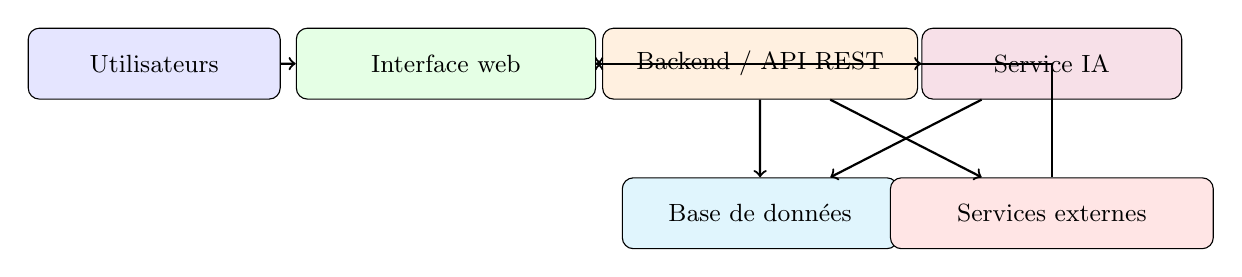
\begin{tikzpicture}[scale=0.95, every node/.style={font=\small}]
    \node[draw, rounded corners, fill=blue!10, minimum width=3.2cm, minimum height=0.9cm] (user) at (1.8,4.0) {Utilisateurs};
    \node[draw, rounded corners, fill=green!10, minimum width=3.8cm, minimum height=0.9cm] (front) at (5.7,4.0) {Interface web};
    \node[draw, rounded corners, fill=orange!12, minimum width=4.0cm, minimum height=0.9cm] (back) at (9.9,4.0) {Backend / API REST};
    \node[draw, rounded corners, fill=purple!12, minimum width=3.3cm, minimum height=0.9cm] (ai) at (13.8,4.0) {Service IA};

    \node[draw, rounded corners, fill=cyan!12, minimum width=3.5cm, minimum height=0.9cm] (data) at (9.9,2.0) {Base de données};
    \node[draw, rounded corners, fill=red!10, minimum width=4.1cm, minimum height=0.9cm] (ext) at (13.8,2.0) {Services externes};

    \draw[->, thick] (user) -- (front);
    \draw[->, thick] (front) -- (back);
    \draw[->, thick] (back) -- (ai);
    \draw[->, thick] (back) -- (data);
    \draw[->, thick] (back) -- (ext);
    \draw[->, thick] (ai) -- (data);
    \draw[->, thick] (ext) |- (front);
\end{tikzpicture}
\caption{Schéma global simplifié de l'architecture du système.}
\label{fig:archi_globale_simple_ch2}
\end{figure}

\noindent
Les elements principaux sont :
\begin{itemize}
    \item \textbf{Interface web} : accès des différents rôles au système ;
    \item \textbf{Backend / API} : gestion des règles métier et de la sécurité ;
    \item \textbf{Service IA} : analyse des images retiniennes et production des resultats ;
    \item \textbf{Base de données} : stockage des comptes, patients, examens et alertes ;
    \item \textbf{Services externes} : notifications et communication temps reel.
\end{itemize}

\subsection{Architecture detaillee (diagrammes de sequence)}
Les diagrammes suivants decrivent les echanges applicatifs sur des scenarios critiques,
avec un accent sur la responsabilité clinique, la traçabilité et la priorisation des cas à risque.

\subsubsection*{Authentification sécurisée et responsabilité clinique}
\begin{figure}[H]
        \centering
        \includegraphics[width=1\\linewidth]{nchlh auth final.png}
    \caption{Diagramme de séquence - Authentification sécurisée et traçabilité d'accès}
\end{figure}
Ce diagramme détaille le contrôle d'accès par rôle, la création de session JWT et la traçabilité des connexions pour sécuriser les actions cliniques et administratives.

\subsubsection*{Création d'examen et orchestration clinique}
\begin{figure}[H]
    \centering
            \includegraphics[width=1\linewidth]{oyaaaaaaaaa.png}
    \caption{Diagramme de séquence - Création d'examen par l'Administrateur de centre}
\end{figure}
Ce diagramme illustre la création d'un examen médical, l'envoi de l'image rétinienne et l'orchestration du flux clinique jusqu'au déclenchement de l'analyse IA.

\subsubsection*{Analyse IA, triage clinique et generation d'alerte}
\begin{figure}[H]
               \centering
               \includegraphics[width=1\linewidth]{zab.pdf4.png}
    \caption{Diagramme de sequence - Analyse IA et priorisation des alertes cliniques}
\end{figure}
Ce diagramme présente l'inférence IA, la production de l'explicabilité (Grad-CAM) et la création d'alertes pour orienter rapidement les cas sévères vers le médecin.

\subsubsection*{Création de centre et attribution d'administration}
\begin{figure}[H]
         \centering
     \includegraphics[width=1\linewidth]{nchlh superfinal.png}
    \caption{Diagramme de séquence - Création de centre et attribution de l'administrateur de centre}
\end{figure}
Ce diagramme décrit la gouvernance plateforme assurée par le Super administrateur : création/configuration de centre, attribution des droits et continuités des opérations cliniques.

\subsection{Hardware environment}
L'environnement materiel requis est defini a deux niveaux.

\subsubsection*{Machine de developpement}
\begin{itemize}
    \item système Windows ou Linux ;
    \item processeur multi-coeurs (classe Intel Core i5/i7 ou equivalent) ;
    \item memoire RAM recommandee : 16 Go ou plus ;
    \item stockage SSD pour accélérer les accès aux datasets/modèles.
\end{itemize}

\subsubsection*{Machine d'execution IA}
\begin{itemize}
    \item CPU moderne pour inference standard ;
    \item GPU optionnel (CUDA) pour acceleration de l'inference et des batchs ;
    \item espace disque suffisant pour modeles, checkpoints et heatmaps.
\end{itemize}

\subsection{Software environment}

\subsubsection*{Development tools}
\begin{itemize}
    \item Visual Studio Code ;
    \item Git/GitHub pour le versioning ;
    \item Postman (ou equivalent) pour tests API ;
    \item scripts Python/Node pour automatisation des taches techniques.
\end{itemize}

\subsubsection*{Frontend environment (framework, design, API communication)}
\begin{itemize}
    \item frontend web en HTML/CSS/JavaScript ;
    \item design responsive pour dashboards Administrateur de centre/Médecin/Super administrateur ;
    \item consommation API backend via requetes HTTP ;
    \item reception des evenements temps reel via WebSocket.
\end{itemize}

\subsubsection*{Backend environment (framework, language, architecture, API type)}
\begin{itemize}
    \item langage : JavaScript (Node.js) ;
    \item framework : Express.js ;
    \item architecture backend modulaire (routes, middleware, services, config) ;
    \item API de type REST sécurisée par JWT.
\end{itemize}

\subsubsection*{AI service environment}
\begin{itemize}
    \item langage : Python ;
    \item framework API : FastAPI ;
    \item bibliotheques IA : PyTorch, TorchVision, OpenCV, Pillow, NumPy ;
    \item execution modele + production heatmap via endpoints dedies.
\end{itemize}

\subsubsection*{Data storage}
\begin{itemize}
    \item base relationnelle legere : SQLite ;
    \item organisation des fichiers images/resultats dans des repertoires structures ;
    \item sauvegarde périodique recommandée pour données critiques.
\end{itemize}

\subsubsection*{Realtime communication}
\begin{itemize}
    \item service WebSocket pour notifications instantanees ;
    \item diffusion sélective des événements selon le rôle ;
    \item synchronisation des dashboards avec l'etat des examens/alertes.
\end{itemize}

\section{Fiches descriptives des cas d'utilisation}
Les fiches suivantes presentent de maniere detaillee et homogeneisee chaque cas d'utilisation principal,
en utilisant une structure coherente : objectif, acteurs, preconditions, scenarios et postconditions.

\subsection{Cas d'utilisation - Administrateur de centre : Orchestration opérationnelle du dépistage clinique}
\begin{table}[H]
\centering
\renewcommand{\arraystretch}{1.3}
\begin{tabular}{|p{5cm}|p{10cm}|}
\hline
\textbf{Nom du cas d'utilisation} & Orchestration opérationnelle du dépistage clinique \\ \hline

\textbf{Objectif} & Permettre à l'Administrateur de centre d'orchestrer les flux de dépistage clinique, de garantir la qualité des données et d'assurer le suivi des demandes de support opérationnel en vue d'optimiser la prise en charge clinique. \\ \hline

\textbf{Acteur principal} & Administrateur de centre \\ \hline

\textbf{Préconditions} & 
\begin{itemize}
\item Administrateur de centre authentifié et connecté au système.
\item Centre actif et accessible.
\end{itemize} \\ \hline

\textbf{Scénario nominal} & 
\begin{itemize}
\item L'Administrateur de centre accede au tableau de bord du centre.
\item Il consulte les dossiers en attente et priorise les examens a demarrer.
\item Il selectionne ou ajoute un patient si necessaire.
\item Il démarre l'examen (création, paramètres et téléversement d'image rétinienne si capture externe).
\item Le système enregistre l'examen et déclenche l'analyse IA automatiquement.
\item L'Administrateur de centre consulte l'etat de l'examen et les resultats IA.
\item Si nécessaire, il accède à la section support et crée une demande d'assistance.
\item Il suit l'etat de la demande de support.
\end{itemize} \\\hline

\textbf{Scénarios alternatifs} &
\begin{itemize}
\item Erreur lors du téléversement de l'image (format invalide, fichier corrompu).
\item Données patient incomplètes (nom, date de naissance manquants).
\item Médecin non disponible au centre.
\item Ticket support non traite ou en attente de reponse prolongee.
\end{itemize} \\ \hline

\textbf{Postconditions} & 
\begin{itemize}
\item L'examen est enregistré dans le système.
\item La demande de support est créée ou mise à jour.
\item L'analyse IA est declenchee ou comfortee.
\end{itemize} \\ \hline
\end{tabular}
\caption{Fiche descriptive - Administrateur de centre (orchestration opérationnelle du dépistage clinique)}
\end{table}

\subsection{Cas d'utilisation - Médecin : Validation diagnostique et prise de décision clinique}
\begin{table}[H]
\centering
\renewcommand{\arraystretch}{1.3}
\begin{tabular}{|p{5cm}|p{10cm}|}
\hline
\textbf{Nom du cas d'utilisation} & Validation diagnostique et prise de décision clinique \\ \hline

\textbf{Objectif} & Permettre au Médecin de valider les prédictions IA, d'interpréter rigoureusement les données cliniques et de prendre une décision thérapeutique éclairée et responsable pour assurer la qualité des soins. \\ \hline

\textbf{Acteur principal} & Médecin \\ \hline

\textbf{Preconditions} & 
\begin{itemize}
\item Médecin authentifié et connecté au système.
\item Examens disponibles et analyses par le service IA.
\end{itemize} \\ \hline

\textbf{Scenario nominal} &
\begin{itemize}
\item Le Médecin se connecte au système et accède au tableau de bord.
\item Le système affiche en priorité les cas sévères (alertes avec grade $\geq 3$).
\item Le Médecin consulte les examens urgents en premier.
\item Il visualise l'image retinienne originale associee a l'examen.
\item Il examine la prediction IA (grade, score de confiance) et la heatmap Grad-CAM.
\item Le Médecin analyse le cas et prend une décision clinique.
\item Il redige le rapport d'examen avec son interpretation clinique.
\item Il consulte l'historique des examens du patient pour suivi longitudinal.
\item Il marque l'alerte comme traitée dans le système.
\item Il télécharge l'examen complet pour archivage ou impression si nécessaire.
\end{itemize} \\ \hline

\textbf{Scenarios alternatifs} &
\begin{itemize}
\item Pas d'images retiniennes disponibles pour consultation.
\item Le modele IA n'a pu generer de prediction (image corrompue ou invalide).
\item Heatmap indisponible ou de mauvaise qualité.
\item Données patient incomplètes ou incohérentes.
\item Alerte déjà traitée par un autre médecin.
\end{itemize} \\ \hline

\textbf{Postconditions} &
\begin{itemize}
\item L'examen est consulte et interprete.
\item Le rapport clinique est redige et enregistre.
\item L'alerte est marquee comme resolue ou redirigee.
\item L'historique du patient est disponible pour suivi.
\end{itemize} \\ \hline
\end{tabular}
\caption{Fiche descriptive - Médecin (validation diagnostique et prise de décision clinique)}
\end{table}

\subsection{Cas d'utilisation - Super administrateur : Pilotage stratégique et supervision clinique globale}
\begin{table}[H]
\centering
\renewcommand{\arraystretch}{1.3}
\begin{tabular}{|p{5cm}|p{10cm}|}
\hline
\textbf{Nom du cas d'utilisation} & Pilotage strategique et supervision clinique globale \\ \hline

\textbf{Objectif} & Assurer la gouvernance globale de la plateforme, superviser les indicateurs cliniques, suivre les centres actifs et garantir la disponibilité ainsi que la fiabilité du système au service de l'excellence médicale. \\ \hline

\textbf{Acteur principal} & Super administrateur \\ \hline

\textbf{Preconditions} &
\begin{itemize}
\item Super administrateur authentifié et connecté au système.
\item Droits d'administration globale confirmes.
\end{itemize} \\ \hline

\textbf{Scenario nominal} &
\begin{itemize}
\item Le Super administrateur accede au tableau de bord global de la plateforme.
\item Il gère la création, la configuration, l'activation et la suspension/désactivation des centres.
\item Il attribue ou retire le statut d'administrateur de centre aux utilisateurs concernes.
\item Il centralise et suit les incidents et demandes d'assistance provenant de tous les centres.
    \item Il priorise les tickets et coordonne leur traitement avec les équipes de support.
    \item Il vérifie la disponibilité et la performance des services critiques (backend, IA, base de données).
\item Il documente les actions et décisions prises pour assurer la traçabilité.
\item Ce rôle est global, distinct d'un administrateur de centre, et pourra évoluer avec de nouvelles responsabilités.
\end{itemize} \\ \hline

\textbf{Scenarios alternatifs} &
\begin{itemize}
\item Un centre ne repond plus (indisponibilite du service).
\item Nombreuses erreurs IA detectees pour une region specifique.
\item Anomalie de performance : ralentissement général du système.
\item Utilisateur avec droits incorrects ou suspects.
\item Stockage disque saturation approchant la limite critique.
\end{itemize} \\ \hline

\textbf{Postconditions} &
\begin{itemize}
\item Les centres sont mis a jour et administres.
\item Les utilisateurs et leurs droits sont valides.
\item Les alertes système sont résolues ou escaladées.
\item Les statistiques et metriques sont documentees.
\end{itemize} \\ \hline
\end{tabular}
\caption{Fiche descriptive - Super administrateur (pilotage stratégique et supervision clinique globale)}
\end{table}

\subsection{Cas d'utilisation - Service IA : Support décisionnel et traçabilité diagnostique}
\begin{table}[H]
\centering
\renewcommand{\arraystretch}{1.3}
\begin{tabular}{|p{5cm}|p{10cm}|}
\hline
\textbf{Nom du cas d'utilisation} & Support décisionnel et traçabilité diagnostique \\ \hline

\textbf{Objectif} & Fournir une analyse automatisée rigoureuse des images rétiniennes, générer des prédictions cliniquement pertinentes avec confiance quantifiée et produire des explications visuelles (Grad-CAM) pour soutenir la décision diagnostique du médecin. \\ \hline

\textbf{Acteur principal} & Service IA (FastAPI + ResNet) \\ \hline

\textbf{Preconditions} &
\begin{itemize}
\item Une image retinienne valide  est disponible.
\item L'examen a été créé dans le système et authentifié.
\item Le modele ResNet est charge et operationnel.
\item Ressources de calcul (CPU/GPU) sont disponibles.
\end{itemize} \\ \hline

\textbf{Scenario nominal} &
\begin{itemize}
\item Le backend envoie l'image retinienne au Service IA via appel HTTP.
\item Le Service IA receptionne l'image et valide son format.
\item L'image est pretraitee (normalisation, redimensionnement, augmentation si necessaire).
\item Le modele ResNet effectue l'inference sur l'image pretraitee.
\item Le système prédit le grade de rétinopathie (0, 1, 2, 3 ou 4).
\item Le score de confiance (probabilite) est calcule a partir des logits.
\item Une heatmap Grad-CAM est générée pour expliquer la décision du modèle.
\item Les resultats (grade, confiance, chemin de la heatmap) sont retournes au backend en format JSON.
\item Le backend enregistre les résultats dans la base de données.
\item Les resultats sont rendus disponibles a l'interface Médecin pour consultation.
\end{itemize} \\ \hline

\textbf{Scenarios alternatifs} &
\begin{itemize}
\item Image invalide ou corrompue : rejet avec message d'erreur.
\item Format d'image non supporte : conversion ou rejet.
\item Echec du modele IA (poids manquants, memoire insuffisante) : erreur HTTP 500.
\item Temps de reponse trop eleve (>30 secondes) : timeout possible du frontend.
\item Heatmap non generee pour raison technique : resultat IA retourne sans heatmap.
\end{itemize} \\ \hline

\textbf{Postconditions} &
\begin{itemize}
\item Les resultats de prediction (grade, confiance, heatmap) sont generes et stockes.
\item Les données sont accessibles pour consultation par le médecin.
\item Un enregistrement de trace (logs) est conserve pour audit et debugging.
\end{itemize} \\ \hline
\end{tabular}
\caption{Fiche descriptive - Service IA (support décisionnel et traçabilité diagnostique)}
\end{table}

\subsection{Cas d'utilisation - Tous les acteurs : Authentification sécurisée et responsabilité clinique}
\begin{table}[H]
\centering
\renewcommand{\arraystretch}{1.3}
\begin{tabular}{|p{5cm}|p{10cm}|}
\hline
\textbf{Nom du cas d'utilisation} & Authentification sécurisée et responsabilité clinique \\ \hline

\textbf{Objectif} & Autoriser les utilisateurs cliniques et administratifs à s'authentifier de manière sécurisée, maintenir la traçabilité des actions dans un contexte réglementaire médicale et terminer leur session de manière fiable. \\ \hline

\textbf{Acteur principal} & Tous les acteurs (Administrateur de centre, Admin, Médecin, Super administrateur) \\ \hline

\textbf{Preconditions} &
\begin{itemize}
\item Compte utilisateur existe et est actif dans le système.
\item Centre affilie (le cas echeant) est actif.
\end{itemize} \\ \hline

\textbf{Scenario nominal} &
\begin{itemize}
\item L'utilisateur accede a la page de connexion.
\item Il saisit ses identifiants (email, mot de passe).
\item Le système valide les identifiants contre la base de données.
\item Le système génère un token JWT sécurisé et stocke la session.
\item L'utilisateur est redirigé vers le tableau de bord correspondant à son rôle.
\item L'utilisateur peut effectuer les actions autorisées par son rôle.
\item L'utilisateur clique sur deconnexion.
\item Le système invalide le token et termine la session.
\item L'utilisateur est redirige vers la page de connexion.
\end{itemize} \\ \hline

\textbf{Scenarios alternatifs} &
\begin{itemize}
\item Identifiants incorrects : message d'erreur et tentative d'authentification.
\item Compte désactivé ou supprimé : refus d'accès.
\item Centre affilié non actif : refus d'accès pour Administrateur de centre/Médecin.
\item Session expieree apres inactivite prolongee : redirection a la connexion.
\item Token invalide ou manipulé : refus d'accès et redirection à la connexion.
\end{itemize} \\ \hline

\textbf{Postconditions} &
\begin{itemize}
\item Utilisateur authentifié et session créée OU utilisateur déconnecté et session terminée.
\item Droits d'accès basés sur le rôle sont appliqués.
\end{itemize} \\ \hline
\end{tabular}
\caption{Fiche descriptive - Authentification et gestion de session}
\end{table}

\section{Conclusion}
Ce chapitre a présenté une spécification complète du système, depuis l'analyse des acteurs
jusqu'a l'architecture technique detaillee. La modelisation proposee garantit une base coherente
pour l'implementation et la validation de la plateforme en contexte reel.

Les fiches descriptives des cas d'utilisation offrent une formalisation rigoureuse et homogeneisee,
facilitant la communication entre les équipes métier, de conception et de développement.

La suite du rapport peut s'appuyer sur ce cadre pour decrire la realisation,
les tests d'integration et l'evaluation finale de la solution.
% =========================

\chapter{Analyse du système et architecture technique}
\label{chap:analyse_architecture}

\section{Introduction}
Ce chapitre formalise la vision système de la plateforme de dépistage automatisé de la rétinopathie diabétique.
Il présente d'abord l'analyse du système (acteurs, exigences), puis la modélisation UML globale,
et enfin l'architecture complete de la solution (logicielle, materielle et operationnelle).

Le contenu est appliqué au projet réalisé, en conservant les rôles métier réels :
\textbf{Administrateur de centre}, \textbf{Admin}, \textbf{Médecin}, \textbf{Super administrateur}, ainsi que l'acteur technique secondaire \textbf{Service IA}.

\section{Analyse du système}

\subsection{Acteurs}
Les acteurs identifiés sont classés en deux catégories : acteurs humains (métier) et acteurs système (techniques).

\subsubsection*{Acteurs humains (Human Actors)}
\begin{itemize}
    \item \textbf{Administrateur de centre} : gère les patients et les médecins du centre, crée les examens,
    envoie les images rétiniennes et consulte l'historique.
    \item \textbf{Admin} : assure l'administration applicative courante (parametrage, suivi operationnel,
    controle des utilisateurs selon les droits attribues).
    \item \textbf{Médecin} : consulte les examens classes par priorite, interprete la prediction IA et la heatmap,
    puis valide la conduite clinique.
    \item \textbf{Super administrateur} : administre les centres, gère la gouvernance globale (comptes, support, supervision,
    disponibilité du système).
\end{itemize}

\subsubsection*{Acteurs système (System Actors)}
\begin{itemize}
    \item \textbf{Service IA} (acteur secondaire principal) : reçoit l'image, exécute l'inférence,
    génère la heatmap Grad-CAM et retourne grade + confiance.
    \item \textbf{Service WebSocket} : diffuse les notifications temps reel (nouveaux examens, alertes severes,
    mises a jour d'etat).
    \item \textbf{Serveur SMTP/SMS} : assure les communications asynchrones (notifications, alertes critiques).
\end{itemize}

\textbf{Note de modelisation :} \textit{Patient} et \textit{Center} ne sont pas des acteurs,
mais des entités métier manipulées par les acteurs humains.

\subsection{Exigences fonctionnelles}
Les exigences fonctionnelles du système sont regroupées par domaine métier.

\subsubsection*{Gestion des comptes et sécurité}
\begin{itemize}
    \item authentification par rôle (Administrateur de centre, Admin, Médecin, Super administrateur) ;
    \item autorisation basée sur le rôle pour chaque route métier ;
    \item gestion de session et deconnexion sécurisée.
\end{itemize}

\subsubsection*{Gestion operationnelle du depistage}
\begin{itemize}
    \item création/modification/consultation/archivage de patients ;
    \item gestion des médecins rattachés à un centre ;
    \item création d'un examen avec téléversement d'image rétinienne ;
    \item association patient-médecin-centre lors de la création d'examen.
\end{itemize}

\subsubsection*{Analyse IA et explicabilité}
\begin{itemize}
    \item envoi de l'image vers le service IA ;
    \item prédiction automatique du grade de rétinopathie (0 à 4) ;
    \item calcul du score de confiance ;
    \item génération et stockage d'une heatmap Grad-CAM ;
    \item restitution du résultat dans l'interface Médecin.
\end{itemize}

\subsubsection*{Alertes et supervision}
\begin{itemize}
    \item création automatique d'alerte pour les cas sévères (grade $\geq 3$) ;
    \item notification temps réel du Médecin ;
    \item suivi de l'état des alertes (nouvelle, en cours, résolue) ;
    \item supervision transversale des centres et du support par le Super administrateur.
\end{itemize}

\subsection{Exigences non fonctionnelles}
Les exigences non fonctionnelles assurent la qualité globale du système en production.

\begin{itemize}
    \item \textbf{Performance} : temps de reponse court pour l'inference et l'affichage ;
    \item \textbf{Disponibilité} : accès continu des interfaces centre, médecin et supervision ;
    \item \textbf{Sécurité} : protection des données médicales, contrôle d'accès et isolation par centre ;
    \item \textbf{Fiabilité} : traçabilité des examens, alertes et actions utilisateurs ;
    \item \textbf{Scalabilite} : possibilite d'augmenter le nombre de centres et le volume d'images ;
    \item \textbf{Maintenabilite} : architecture modulaire (frontend, backend, IA, realtime) ;
    \item \textbf{Explicabilité} : visualisation interprétable (Grad-CAM) pour appuyer la décision clinique.
\end{itemize}

\section{Modélisation du système}

\subsection{Diagramme de cas d'utilisation général}
Le diagramme suivant represente la vue fonctionnelle globale avec
quatre acteurs primaires (Administrateur de centre, Admin, Médecin, Super administrateur) et un acteur secondaire (Service IA).

\begin{figure}[H]
\centering
\begin{tikzpicture}[scale=0.86, every node/.style={font=\small}]
    % Limite système
    \draw[thick] (1.8,0.6) rectangle (13.0,8.4);
    \node[anchor=west] at (2.0,8.1) {Système de dépistage RD};

    % Acteurs gauche
    % Administrateur de centre
    \draw (0.3,6.7) circle (0.25);
    \draw (0.3,6.45) -- (0.3,5.7);
    \draw (-0.2,6.05) -- (0.8,6.05);
    \draw (0.3,5.7) -- (-0.05,5.1);
    \draw (0.3,5.7) -- (0.65,5.1);
    \node at (0.3,4.8) {Administrateur de centre};

    % Admin
    \draw (-1.0,4.8) circle (0.25);
    \draw (-1.0,4.55) -- (-1.0,3.8);
    \draw (-1.5,4.15) -- (-0.5,4.15);
    \draw (-1.0,3.8) -- (-1.35,3.2);
    \draw (-1.0,3.8) -- (-0.65,3.2);
    \node at (-1.0,2.9) {Admin};

    % Médecin
    \draw (0.3,4.2) circle (0.25);
    \draw (0.3,3.95) -- (0.3,3.2);
    \draw (-0.2,3.55) -- (0.8,3.55);
    \draw (0.3,3.2) -- (-0.05,2.6);
    \draw (0.3,3.2) -- (0.65,2.6);
    \node at (0.3,2.3) {Médecin};

    % Super administrateur
    \draw (0.3,1.8) circle (0.25);
    \draw (0.3,1.55) -- (0.3,0.8);
    \draw (-0.2,1.15) -- (0.8,1.15);
    \draw (0.3,0.8) -- (-0.05,0.25);
    \draw (0.3,0.8) -- (0.65,0.25);
    \node at (0.3,-0.05) {Super administrateur};

    % Acteur secondaire droite : Service IA
    \draw (14.4,4.4) circle (0.25);
    \draw (14.4,4.15) -- (14.4,3.4);
    \draw (13.9,3.8) -- (14.9,3.8);
    \draw (14.4,3.4) -- (14.05,2.8);
    \draw (14.4,3.4) -- (14.75,2.8);
    \node at (14.4,2.45) {Service IA};

    % Use cases
    \node[draw, ellipse, minimum width=4.7cm, minimum height=0.85cm] (u1) at (5.5,7.3) {Se connecter};
    \node[draw, ellipse, minimum width=4.7cm, minimum height=0.85cm] (u2) at (5.5,6.2) {Gérer patients};
    \node[draw, ellipse, minimum width=4.7cm, minimum height=0.85cm] (u3) at (5.5,5.1) {Gérer médecins};
    \node[draw, ellipse, minimum width=4.7cm, minimum height=0.85cm] (u4) at (5.5,4.0) {Créer examen};
    \node[draw, ellipse, minimum width=4.7cm, minimum height=0.85cm] (u5) at (5.5,2.9) {Consulter historique};
    \node[draw, ellipse, minimum width=4.7cm, minimum height=0.85cm] (u6) at (9.4,5.8) {Consulter examens et alertes};
    \node[draw, ellipse, minimum width=4.7cm, minimum height=0.85cm] (u7) at (9.4,4.5) {Interpreter prediction + heatmap};
    \node[draw, ellipse, minimum width=4.7cm, minimum height=0.85cm] (u8) at (9.4,3.2) {Superviser centres et support};
    \node[draw, ellipse, minimum width=4.7cm, minimum height=0.85cm] (u9) at (9.4,1.9) {Administrer comptes globaux};
    \node[draw, ellipse, minimum width=4.7cm, minimum height=0.85cm] (u10) at (7.5,0.95) {Se déconnecter};
    \node[draw, ellipse, minimum width=4.7cm, minimum height=0.85cm] (u11) at (11.0,6.95) {Analyser image rétinienne};

    % Liens Administrateur de centre
    \draw (0.8,6.05) -- (u1.west);
    \draw (0.8,6.05) -- (u2.west);
    \draw (0.8,6.05) -- (u3.west);
    \draw (0.8,6.05) -- (u4.west);
    \draw (0.8,6.05) -- (u5.west);
    \draw (0.8,6.05) -- (u10.west);

    % Liens Médecin
    \draw (0.8,3.55) -- (u1.west);
    \draw (0.8,3.55) -- (u6.west);
    \draw (0.8,3.55) -- (u7.west);
    \draw (0.8,3.55) -- (u10.west);

    % Liens Admin
    \draw (-0.5,4.15) -- (u1.west);
    \draw (-0.5,4.15) -- (u2.west);
    \draw (-0.5,4.15) -- (u3.west);
    \draw (-0.5,4.15) -- (u5.west);
    \draw (-0.5,4.15) -- (u10.west);

    % Liens Super administrateur
    \draw (0.8,1.15) -- (u1.west);
    \draw (0.8,1.15) -- (u8.west);
    \draw (0.8,1.15) -- (u9.west);
    \draw (0.8,1.15) -- (u10.west);

    % Include vers IA
    \draw[->, dashed] (u4.east) -- (u11.west);
    \node at (8.6,6.6) {<<include>>};
    \draw[->, dashed] (u7.north) -- (u11.south);
    \node at (10.3,5.9) {<<include>>};

    % Lien acteur IA
    \draw (13.9,3.8) -- (u11.east);
\end{tikzpicture}
\caption{Diagramme de cas d'utilisation général du système.}
\label{fig:usecase_general_ch2}
\end{figure}

\subsection{Diagramme de classes general}
Le diagramme de classes ci-dessous montre les principales entités métier,
les specialisations de l'utilisateur et les relations entre objets applicatifs

\begin{figure}[H]
\centering
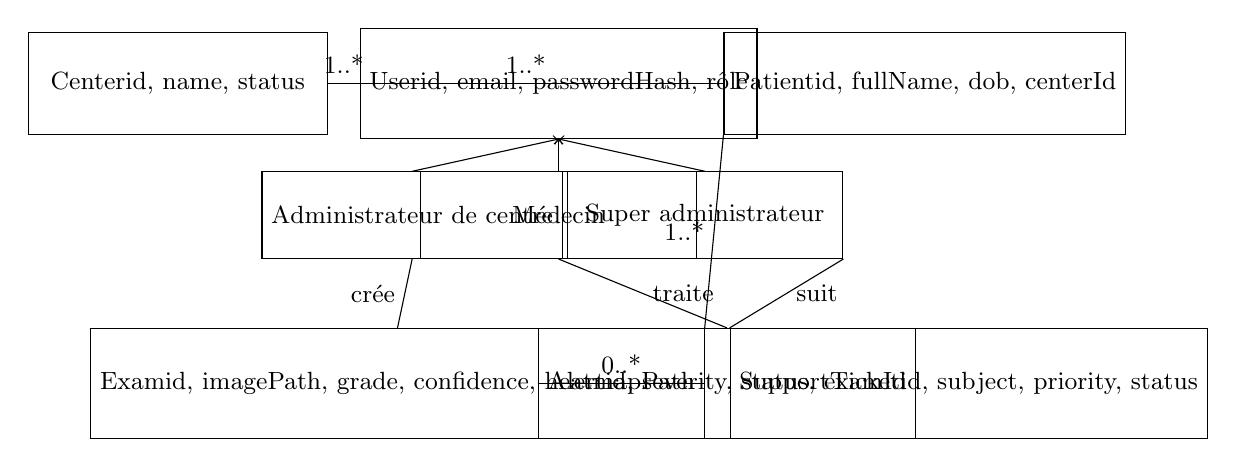
\begin{tikzpicture}[scale=0.93, every node/.style={font=\small}]
    % Classes principales
    \node[draw, rectangle, minimum width=3.8cm, minimum height=1.3cm] (center) at (2.0,7.0) {Center\\id, name, status};
    \node[draw, rectangle, minimum width=3.8cm, minimum height=1.4cm] (user) at (7.2,7.0) {User\\id, email, passwordHash, rôle};
    \node[draw, rectangle, minimum width=3.8cm, minimum height=1.3cm] (patient) at (12.2,7.0) {Patient\\id, fullName, dob, centerId};

    \node[draw, rectangle, minimum width=3.5cm, minimum height=1.1cm] (ca) at (5.2,5.2) {Administrateur de centre};
    \node[draw, rectangle, minimum width=3.5cm, minimum height=1.1cm] (doc) at (7.2,5.2) {Médecin};
    \node[draw, rectangle, minimum width=3.5cm, minimum height=1.1cm] (sa) at (9.2,5.2) {Super administrateur};

    \node[draw, rectangle, minimum width=4.0cm, minimum height=1.4cm] (exam) at (5.0,2.9) {Exam\\id, imagePath, grade, confidence, heatmapPath};
    \node[draw, rectangle, minimum width=4.0cm, minimum height=1.4cm] (alert) at (9.5,2.9) {Alert\\id, severity, status, examId};
    \node[draw, rectangle, minimum width=4.3cm, minimum height=1.4cm] (ticket) at (12.8,2.9) {SupportTicket\\id, subject, priority, status};

    % Relations
    \draw (center.east) -- node[above] {1..*} (user.west);
    \draw (center.east) -- node[above] {1..*} (patient.west);

    % Generalisation
    \draw[->] (ca.north) -- (user.south);
    \draw[->] (doc.north) -- (user.south);
    \draw[->] (sa.north) -- (user.south);

    \draw (patient.south west) -- node[left] {1..*} (exam.north east);
    \draw (ca.south) -- node[left] {crée} (exam.north);
    \draw (doc.south) -- node[right] {traite} (alert.north);
    \draw (exam.east) -- node[above] {0..*} (alert.west);
    \draw (sa.south east) -- node[right] {suit} (ticket.north west);
\end{tikzpicture}
\caption{Diagramme de classes general de la plateforme.}
\label{fig:class_general_ch2}
\end{figure}

\section{Architecture complète du système}

\subsection{Architecture du système (schéma global)}
Le schema global presente les couches logiques principales et les flux inter-services.

\begin{figure}[H]
\centering
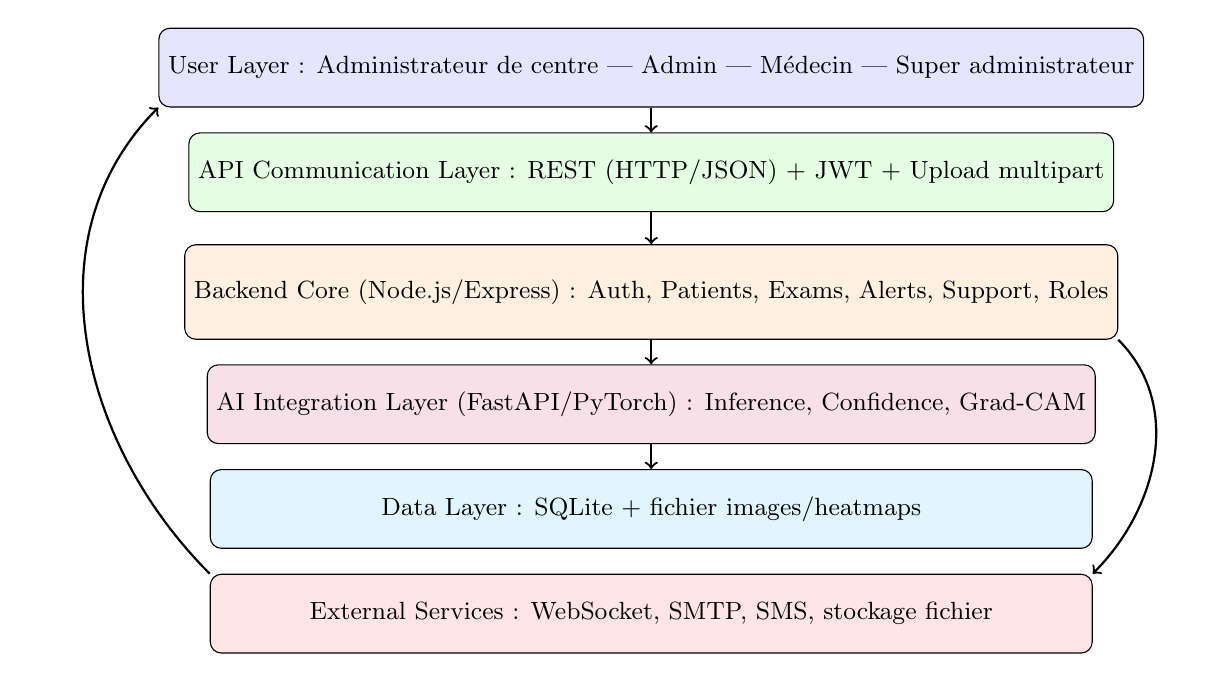
\begin{tikzpicture}[scale=0.95, every node/.style={font=\small}]
    \node[draw, rounded corners, fill=blue!10, minimum width=11.2cm, minimum height=1.0cm] (u) at (7.0,8.0) {User Layer : Administrateur de centre | Admin | Médecin | Super administrateur};
    \node[draw, rounded corners, fill=green!10, minimum width=11.2cm, minimum height=1.0cm] (api) at (7.0,6.6) {API Communication Layer : REST (HTTP/JSON) + JWT + Upload multipart};
    \node[draw, rounded corners, fill=orange!12, minimum width=11.2cm, minimum height=1.2cm] (core) at (7.0,5.0) {Backend Core (Node.js/Express) : Auth, Patients, Exams, Alerts, Support, Roles};
    \node[draw, rounded corners, fill=purple!12, minimum width=11.2cm, minimum height=1.0cm] (ai) at (7.0,3.5) {AI Integration Layer (FastAPI/PyTorch) : Inference, Confidence, Grad-CAM};
    \node[draw, rounded corners, fill=cyan!12, minimum width=11.2cm, minimum height=1.0cm] (data) at (7.0,2.1) {Data Layer : SQLite + fichier images/heatmaps};
    \node[draw, rounded corners, fill=red!10, minimum width=11.2cm, minimum height=1.0cm] (ext) at (7.0,0.7) {External Services : WebSocket, SMTP, SMS, stockage fichier};

    \draw[->, thick] (u.south) -- (api.north);
    \draw[->, thick] (api.south) -- (core.north);
    \draw[->, thick] (core.south) -- (ai.north);
    \draw[->, thick] (ai.south) -- (data.north);
    \draw[->, thick] (core.south east) to[out=-45,in=45] (ext.north east);
    \draw[->, thick] (ext.north west) to[out=135,in=-135] (u.south west);
\end{tikzpicture}
\caption{Schéma global de l'architecture du système.}
\label{fig:archi_globale_ch2}
\end{figure}

\subsection{Architecture globale de la plateforme}
L'architecture globale du système suit un enchaînement simple et lisible : les utilisateurs accèdent à l'interface web, les requêtes passent par l'API du backend, le service IA traite les images rétiniennes, puis les données et résultats sont stockés et diffusés aux différents rôles.

\begin{figure}[H]
\centering
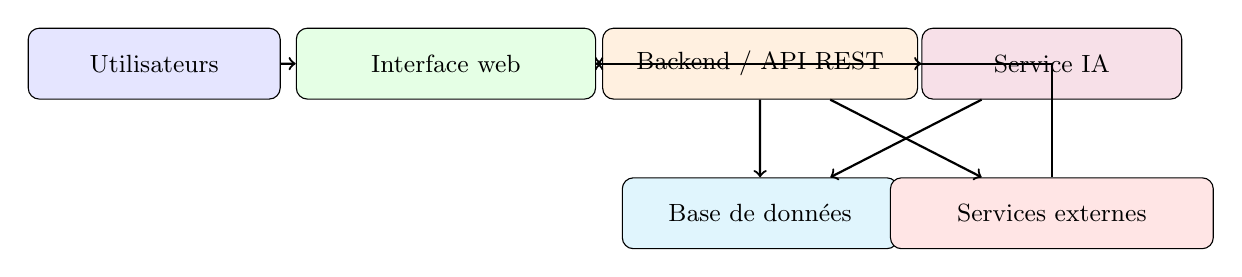
\begin{tikzpicture}[scale=0.95, every node/.style={font=\small}]
    \node[draw, rounded corners, fill=blue!10, minimum width=3.2cm, minimum height=0.9cm] (user) at (1.8,4.0) {Utilisateurs};
    \node[draw, rounded corners, fill=green!10, minimum width=3.8cm, minimum height=0.9cm] (front) at (5.7,4.0) {Interface web};
    \node[draw, rounded corners, fill=orange!12, minimum width=4.0cm, minimum height=0.9cm] (back) at (9.9,4.0) {Backend / API REST};
    \node[draw, rounded corners, fill=purple!12, minimum width=3.3cm, minimum height=0.9cm] (ai) at (13.8,4.0) {Service IA};

    \node[draw, rounded corners, fill=cyan!12, minimum width=3.5cm, minimum height=0.9cm] (data) at (9.9,2.0) {Base de données};
    \node[draw, rounded corners, fill=red!10, minimum width=4.1cm, minimum height=0.9cm] (ext) at (13.8,2.0) {Services externes};

    \draw[->, thick] (user) -- (front);
    \draw[->, thick] (front) -- (back);
    \draw[->, thick] (back) -- (ai);
    \draw[->, thick] (back) -- (data);
    \draw[->, thick] (back) -- (ext);
    \draw[->, thick] (ai) -- (data);
    \draw[->, thick] (ext) |- (front);
\end{tikzpicture}
\caption{Schéma global simplifié de l'architecture du système.}
\label{fig:archi_globale_simple_ch2}
\end{figure}

\noindent
Les elements principaux sont :
\begin{itemize}
    \item \textbf{Interface web} : accès des différents rôles au système ;
    \item \textbf{Backend / API} : gestion des règles métier et de la sécurité ;
    \item \textbf{Service IA} : analyse des images retiniennes et production des resultats ;
    \item \textbf{Base de données} : stockage des comptes, patients, examens et alertes ;
    \item \textbf{Services externes} : notifications et communication temps reel.
\end{itemize}

\subsection{Architecture detaillee (diagrammes de sequence)}
Les diagrammes suivants decrivent les echanges applicatifs sur des scenarios critiques,
avec un accent sur la responsabilité clinique, la traçabilité et la priorisation des cas à risque.

\subsubsection*{Authentification sécurisée et responsabilité clinique}
\begin{figure}[H]
        \centering
        \includegraphics[width=1\\linewidth]{nchlh auth final.png}
    \caption{Diagramme de séquence - Authentification sécurisée et traçabilité d'accès}
\end{figure}
Ce diagramme détaille le contrôle d'accès par rôle, la création de session JWT et la traçabilité des connexions pour sécuriser les actions cliniques et administratives.

\subsubsection*{Création d'examen et orchestration clinique}
\begin{figure}[H]
    \centering
            \includegraphics[width=1\linewidth]{oyaaaaaaaaa.png}
    \caption{Diagramme de séquence - Création d'examen par l'Administrateur de centre}
\end{figure}
Ce diagramme illustre la création d'un examen médical, l'envoi de l'image rétinienne et l'orchestration du flux clinique jusqu'au déclenchement de l'analyse IA.

\subsubsection*{Analyse IA, triage clinique et generation d'alerte}
\begin{figure}[H]
               \centering
               \includegraphics[width=1\linewidth]{zab.pdf4.png}
    \caption{Diagramme de sequence - Analyse IA et priorisation des alertes cliniques}
\end{figure}
Ce diagramme présente l'inférence IA, la production de l'explicabilité (Grad-CAM) et la création d'alertes pour orienter rapidement les cas sévères vers le médecin.

\subsubsection*{Création de centre et attribution d'administration}
\begin{figure}[H]
         \centering
     \includegraphics[width=1\linewidth]{nchlh superfinal.png}
    \caption{Diagramme de séquence - Création de centre et attribution de l'administrateur de centre}
\end{figure}
Ce diagramme décrit la gouvernance plateforme assurée par le Super administrateur : création/configuration de centre, attribution des droits et continuités des opérations cliniques.

\subsection{Hardware environment}
L'environnement materiel requis est defini a deux niveaux.

\subsubsection*{Machine de developpement}
\begin{itemize}
    \item système Windows ou Linux ;
    \item processeur multi-coeurs (classe Intel Core i5/i7 ou equivalent) ;
    \item memoire RAM recommandee : 16 Go ou plus ;
    \item stockage SSD pour accélérer les accès aux datasets/modèles.
\end{itemize}

\subsubsection*{Machine d'execution IA}
\begin{itemize}
    \item CPU moderne pour inference standard ;
    \item GPU optionnel (CUDA) pour acceleration de l'inference et des batchs ;
    \item espace disque suffisant pour modeles, checkpoints et heatmaps.
\end{itemize}

\subsection{Software environment}

\subsubsection*{Development tools}
\begin{itemize}
    \item Visual Studio Code ;
    \item Git/GitHub pour le versioning ;
    \item Postman (ou equivalent) pour tests API ;
    \item scripts Python/Node pour automatisation des taches techniques.
\end{itemize}

\subsubsection*{Frontend environment (framework, design, API communication)}
\begin{itemize}
    \item frontend web en HTML/CSS/JavaScript ;
    \item design responsive pour dashboards Administrateur de centre/Médecin/Super administrateur ;
    \item consommation API backend via requetes HTTP ;
    \item reception des evenements temps reel via WebSocket.
\end{itemize}

\subsubsection*{Backend environment (framework, language, architecture, API type)}
\begin{itemize}
    \item langage : JavaScript (Node.js) ;
    \item framework : Express.js ;
    \item architecture backend modulaire (routes, middleware, services, config) ;
    \item API de type REST sécurisée par JWT.
\end{itemize}

\subsubsection*{AI service environment}
\begin{itemize}
    \item langage : Python ;
    \item framework API : FastAPI ;
    \item bibliotheques IA : PyTorch, TorchVision, OpenCV, Pillow, NumPy ;
    \item execution modele + production heatmap via endpoints dedies.
\end{itemize}

\subsubsection*{Data storage}
\begin{itemize}
    \item base relationnelle legere : SQLite ;
    \item organisation des fichiers images/resultats dans des repertoires structures ;
    \item sauvegarde périodique recommandée pour données critiques.
\end{itemize}

\subsubsection*{Realtime communication}
\begin{itemize}
    \item service WebSocket pour notifications instantanees ;
    \item diffusion sélective des événements selon le rôle ;
    \item synchronisation des dashboards avec l'etat des examens/alertes.
\end{itemize}

\section{Fiches descriptives des cas d'utilisation}
Les fiches suivantes presentent de maniere detaillee et homogeneisee chaque cas d'utilisation principal,
en utilisant une structure coherente : objectif, acteurs, preconditions, scenarios et postconditions.

\subsection{Cas d'utilisation - Administrateur de centre : Orchestration opérationnelle du dépistage clinique}
\begin{table}[H]
\centering
\renewcommand{\arraystretch}{1.3}
\begin{tabular}{|p{5cm}|p{10cm}|}
\hline
\textbf{Nom du cas d'utilisation} & Orchestration opérationnelle du dépistage clinique \\ \hline

\textbf{Objectif} & Permettre à l'Administrateur de centre d'orchestrer les flux de dépistage clinique, de garantir la qualité des données et d'assurer le suivi des demandes de support opérationnel en vue d'optimiser la prise en charge clinique. \\ \hline

\textbf{Acteur principal} & Administrateur de centre \\ \hline

\textbf{Préconditions} & 
\begin{itemize}
\item Administrateur de centre authentifié et connecté au système.
\item Centre actif et accessible.
\end{itemize} \\ \hline

\textbf{Scénario nominal} & 
\begin{itemize}
\item L'Administrateur de centre accede au tableau de bord du centre.
\item Il consulte les dossiers en attente et priorise les examens a demarrer.
\item Il selectionne ou ajoute un patient si necessaire.
\item Il démarre l'examen (création, paramètres et téléversement d'image rétinienne si capture externe).
\item Le système enregistre l'examen et déclenche l'analyse IA automatiquement.
\item L'Administrateur de centre consulte l'etat de l'examen et les resultats IA.
\item Si nécessaire, il accède à la section support et crée une demande d'assistance.
\item Il suit l'etat de la demande de support.
\end{itemize} \\\hline

\textbf{Scénarios alternatifs} &
\begin{itemize}
\item Erreur lors du téléversement de l'image (format invalide, fichier corrompu).
\item Données patient incomplètes (nom, date de naissance manquants).
\item Médecin non disponible au centre.
\item Ticket support non traite ou en attente de reponse prolongee.
\end{itemize} \\ \hline

\textbf{Postconditions} & 
\begin{itemize}
\item L'examen est enregistré dans le système.
\item La demande de support est créée ou mise à jour.
\item L'analyse IA est declenchee ou comfortee.
\end{itemize} \\ \hline
\end{tabular}
\caption{Fiche descriptive - Administrateur de centre (orchestration opérationnelle du dépistage clinique)}
\end{table}

\subsection{Cas d'utilisation - Médecin : Validation diagnostique et prise de décision clinique}
\begin{table}[H]
\centering
\renewcommand{\arraystretch}{1.3}
\begin{tabular}{|p{5cm}|p{10cm}|}
\hline
\textbf{Nom du cas d'utilisation} & Validation diagnostique et prise de décision clinique \\ \hline

\textbf{Objectif} & Permettre au Médecin de valider les prédictions IA, d'interpréter rigoureusement les données cliniques et de prendre une décision thérapeutique éclairée et responsable pour assurer la qualité des soins. \\ \hline

\textbf{Acteur principal} & Médecin \\ \hline

\textbf{Preconditions} & 
\begin{itemize}
\item Médecin authentifié et connecté au système.
\item Examens disponibles et analyses par le service IA.
\end{itemize} \\ \hline

\textbf{Scenario nominal} &
\begin{itemize}
\item Le Médecin se connecte au système et accède au tableau de bord.
\item Le système affiche en priorité les cas sévères (alertes avec grade $\geq 3$).
\item Le Médecin consulte les examens urgents en premier.
\item Il visualise l'image retinienne originale associee a l'examen.
\item Il examine la prediction IA (grade, score de confiance) et la heatmap Grad-CAM.
\item Le Médecin analyse le cas et prend une décision clinique.
\item Il redige le rapport d'examen avec son interpretation clinique.
\item Il consulte l'historique des examens du patient pour suivi longitudinal.
\item Il marque l'alerte comme traitée dans le système.
\item Il télécharge l'examen complet pour archivage ou impression si nécessaire.
\end{itemize} \\ \hline

\textbf{Scenarios alternatifs} &
\begin{itemize}
\item Pas d'images retiniennes disponibles pour consultation.
\item Le modele IA n'a pu generer de prediction (image corrompue ou invalide).
\item Heatmap indisponible ou de mauvaise qualité.
\item Données patient incomplètes ou incohérentes.
\item Alerte déjà traitée par un autre médecin.
\end{itemize} \\ \hline

\textbf{Postconditions} &
\begin{itemize}
\item L'examen est consulte et interprete.
\item Le rapport clinique est redige et enregistre.
\item L'alerte est marquee comme resolue ou redirigee.
\item L'historique du patient est disponible pour suivi.
\end{itemize} \\ \hline
\end{tabular}
\caption{Fiche descriptive - Médecin (validation diagnostique et prise de décision clinique)}
\end{table}

\subsection{Cas d'utilisation - Super administrateur : Pilotage stratégique et supervision clinique globale}
\begin{table}[H]
\centering
\renewcommand{\arraystretch}{1.3}
\begin{tabular}{|p{5cm}|p{10cm}|}
\hline
\textbf{Nom du cas d'utilisation} & Pilotage strategique et supervision clinique globale \\ \hline

\textbf{Objectif} & Assurer la gouvernance globale de la plateforme, superviser les indicateurs cliniques, suivre les centres actifs et garantir la disponibilité ainsi que la fiabilité du système au service de l'excellence médicale. \\ \hline

\textbf{Acteur principal} & Super administrateur \\ \hline

\textbf{Preconditions} &
\begin{itemize}
\item Super administrateur authentifié et connecté au système.
\item Droits d'administration globale confirmes.
\end{itemize} \\ \hline

\textbf{Scenario nominal} &
\begin{itemize}
\item Le Super administrateur accede au tableau de bord global de la plateforme.
\item Il gère la création, la configuration, l'activation et la suspension/désactivation des centres.
\item Il attribue ou retire le statut d'administrateur de centre aux utilisateurs concernes.
\item Il centralise et suit les incidents et demandes d'assistance provenant de tous les centres.
    \item Il priorise les tickets et coordonne leur traitement avec les équipes de support.
    \item Il vérifie la disponibilité et la performance des services critiques (backend, IA, base de données).
\item Il documente les actions et décisions prises pour assurer la traçabilité.
\item Ce rôle est global, distinct d'un administrateur de centre, et pourra évoluer avec de nouvelles responsabilités.
\end{itemize} \\ \hline

\textbf{Scenarios alternatifs} &
\begin{itemize}
\item Un centre ne repond plus (indisponibilite du service).
\item Nombreuses erreurs IA detectees pour une region specifique.
\item Anomalie de performance : ralentissement général du système.
\item Utilisateur avec droits incorrects ou suspects.
\item Stockage disque saturation approchant la limite critique.
\end{itemize} \\ \hline

\textbf{Postconditions} &
\begin{itemize}
\item Les centres sont mis a jour et administres.
\item Les utilisateurs et leurs droits sont valides.
\item Les alertes système sont résolues ou escaladées.
\item Les statistiques et metriques sont documentees.
\end{itemize} \\ \hline
\end{tabular}
\caption{Fiche descriptive - Super administrateur (pilotage stratégique et supervision clinique globale)}
\end{table}

\subsection{Cas d'utilisation - Service IA : Support décisionnel et traçabilité diagnostique}
\begin{table}[H]
\centering
\renewcommand{\arraystretch}{1.3}
\begin{tabular}{|p{5cm}|p{10cm}|}
\hline
\textbf{Nom du cas d'utilisation} & Support décisionnel et traçabilité diagnostique \\ \hline

\textbf{Objectif} & Fournir une analyse automatisée rigoureuse des images rétiniennes, générer des prédictions cliniquement pertinentes avec confiance quantifiée et produire des explications visuelles (Grad-CAM) pour soutenir la décision diagnostique du médecin. \\ \hline

\textbf{Acteur principal} & Service IA (FastAPI + ResNet) \\ \hline

\textbf{Preconditions} &
\begin{itemize}
\item Une image retinienne valide  est disponible.
\item L'examen a été créé dans le système et authentifié.
\item Le modele ResNet est charge et operationnel.
\item Ressources de calcul (CPU/GPU) sont disponibles.
\end{itemize} \\ \hline

\textbf{Scenario nominal} &
\begin{itemize}
\item Le backend envoie l'image retinienne au Service IA via appel HTTP.
\item Le Service IA receptionne l'image et valide son format.
\item L'image est pretraitee (normalisation, redimensionnement, augmentation si necessaire).
\item Le modele ResNet effectue l'inference sur l'image pretraitee.
\item Le système prédit le grade de rétinopathie (0, 1, 2, 3 ou 4).
\item Le score de confiance (probabilite) est calcule a partir des logits.
\item Une heatmap Grad-CAM est générée pour expliquer la décision du modèle.
\item Les resultats (grade, confiance, chemin de la heatmap) sont retournes au backend en format JSON.
\item Le backend enregistre les résultats dans la base de données.
\item Les resultats sont rendus disponibles a l'interface Médecin pour consultation.
\end{itemize} \\ \hline

\textbf{Scenarios alternatifs} &
\begin{itemize}
\item Image invalide ou corrompue : rejet avec message d'erreur.
\item Format d'image non supporte : conversion ou rejet.
\item Echec du modele IA (poids manquants, memoire insuffisante) : erreur HTTP 500.
\item Temps de reponse trop eleve (>30 secondes) : timeout possible du frontend.
\item Heatmap non generee pour raison technique : resultat IA retourne sans heatmap.
\end{itemize} \\ \hline

\textbf{Postconditions} &
\begin{itemize}
\item Les resultats de prediction (grade, confiance, heatmap) sont generes et stockes.
\item Les données sont accessibles pour consultation par le médecin.
\item Un enregistrement de trace (logs) est conserve pour audit et debugging.
\end{itemize} \\ \hline
\end{tabular}
\caption{Fiche descriptive - Service IA (support décisionnel et traçabilité diagnostique)}
\end{table}

\subsection{Cas d'utilisation - Tous les acteurs : Authentification sécurisée et responsabilité clinique}
\begin{table}[H]
\centering
\renewcommand{\arraystretch}{1.3}
\begin{tabular}{|p{5cm}|p{10cm}|}
\hline
\textbf{Nom du cas d'utilisation} & Authentification sécurisée et responsabilité clinique \\ \hline

\textbf{Objectif} & Autoriser les utilisateurs cliniques et administratifs à s'authentifier de manière sécurisée, maintenir la traçabilité des actions dans un contexte réglementaire médicale et terminer leur session de manière fiable. \\ \hline

\textbf{Acteur principal} & Tous les acteurs (Administrateur de centre, Admin, Médecin, Super administrateur) \\ \hline

\textbf{Preconditions} &
\begin{itemize}
\item Compte utilisateur existe et est actif dans le système.
\item Centre affilie (le cas echeant) est actif.
\end{itemize} \\ \hline

\textbf{Scenario nominal} &
\begin{itemize}
\item L'utilisateur accede a la page de connexion.
\item Il saisit ses identifiants (email, mot de passe).
\item Le système valide les identifiants contre la base de données.
\item Le système génère un token JWT sécurisé et stocke la session.
\item L'utilisateur est redirigé vers le tableau de bord correspondant à son rôle.
\item L'utilisateur peut effectuer les actions autorisées par son rôle.
\item L'utilisateur clique sur deconnexion.
\item Le système invalide le token et termine la session.
\item L'utilisateur est redirige vers la page de connexion.
\end{itemize} \\ \hline

\textbf{Scenarios alternatifs} &
\begin{itemize}
\item Identifiants incorrects : message d'erreur et tentative d'authentification.
\item Compte désactivé ou supprimé : refus d'accès.
\item Centre affilié non actif : refus d'accès pour Administrateur de centre/Médecin.
\item Session expieree apres inactivite prolongee : redirection a la connexion.
\item Token invalide ou manipulé : refus d'accès et redirection à la connexion.
\end{itemize} \\ \hline

\textbf{Postconditions} &
\begin{itemize}
\item Utilisateur authentifié et session créée OU utilisateur déconnecté et session terminée.
\item Droits d'accès basés sur le rôle sont appliqués.
\end{itemize} \\ \hline
\end{tabular}
\caption{Fiche descriptive - Authentification et gestion de session}
\end{table}

\section{Conclusion}
Ce chapitre a présenté une spécification complète du système, depuis l'analyse des acteurs
jusqu'a l'architecture technique detaillee. La modelisation proposee garantit une base coherente
pour l'implementation et la validation de la plateforme en contexte reel.

Les fiches descriptives des cas d'utilisation offrent une formalisation rigoureuse et homogeneisee,
facilitant la communication entre les équipes métier, de conception et de développement.

La suite du rapport peut s'appuyer sur ce cadre pour decrire la realisation,
les tests d'integration et l'evaluation finale de la solution.